\documentclass{article}

\usepackage[utf8]{inputenc}

\usepackage{amsmath, bm}
\usepackage{graphicx}
\usepackage{amssymb}
\usepackage{float}
\usepackage{caption}
\usepackage{subcaption}
\usepackage{hyperref}
\usepackage{tikz}
\usepackage{layout}
\usepackage{booktabs}

\usepackage[margin=1in]{geometry}
\usepackage{listings}
\usepackage{xcolor}
\usepackage{color, colortbl}
\usepackage{textgreek}
\usepackage{mathrsfs}
\usepackage{savetrees}[moderate]
\usepackage{dirtree}


\usetikzlibrary{calc}
\usetikzlibrary{angles,quotes} % for pic
\usetikzlibrary{patterns,snakes}
\usetikzlibrary{arrows}
\tikzset{>=latex} % for LaTeX arrow head

\setlength{\parskip}{\baselineskip}%
\setlength{\parindent}{0pt}%
\linespread{0.9}


\definecolor{codegreen}{rgb}{0,0.6,0}
\definecolor{codegray}{rgb}{0.5,0.5,0.5}
\definecolor{codepurple}{rgb}{0.58,0,0.82}
\definecolor{backcolour}{rgb}{0.95,0.95,0.92}

\lstdefinestyle{mystyle}{
    backgroundcolor=\color{backcolour},   
    commentstyle=\color{codegreen},
    keywordstyle=\color{magenta},
    numberstyle=\tiny\color{codegray},
    stringstyle=\color{codepurple},
    basicstyle=\ttfamily\footnotesize,
    breakatwhitespace=false,         
    breaklines=true,                 
    captionpos=b,                    
    keepspaces=true,                 
    numbers=left,                    
    numbersep=5pt,                  
    showspaces=false,                
    showstringspaces=false,
    showtabs=false,                  
    tabsize=2
}

\lstset{style=mystyle}



\begin{document}

\title{Computational Fluid Dynamics \\
    \large Final Report}
\author{lwp26}
\date{December 2024}
\maketitle 

\section{Software}
% monumental amount of work required here
\subsection{Modifications}
% interpolate
% write_settings python

Some corrections were made to the code supplied by the course.
The first correction was to the \texttt{interpolate} fortran function to fix an issue which only presented when compiling the program without debug symbols and so was difficult to identify.
It was found that in some cases this function was returning unset memory values at the last point of the array. This is believed to be due to more relaxed precision in \texttt{si} which left it outside the normalised range of \texttt{si\_a}.
The fix was to add a check to see if \texttt{si} is outside the input range, and if so return the boundary value.
A mistake in the python function \texttt{write\_settings} was also found where the gas constants were being written in the incorrect order.

The general program \texttt{stopit} file was removed and replaced with the variable \texttt{av\%crashed} which is set to true if \texttt{NaN} is detected, or if the user interrupts the program.
Not only is this more efficient, but also now allows cases to be run in parallel writing only to case specific files, and not a shared program file which causes write violations.
This was imporant to accelerate the testing and a custom python thread pool manager was written for this purpose.
A worker creates the directory structure for the case, runs the solver, and then writes the key results to a shared file.
The worker directory and run function are shown in the appendix \ref{fig:worker_dir}.
The number of threads in the threadpool was set to 8, less than the number of cores on the machine to prevent incorrect time measurements due to windows thread scheduling.

The GUI was improved with more inputs and improved visualisation animations.
The zoom and pan no longer resets on each frame update and is consistent between tabs.


\subsection{Improvements}
% runge kutta
% deferred correction
% residual averaging
% spatially varying timestep
\subsubsection{Runge-Kutta}

The Runge-Kutta methods are a family of implicit and explicit iterative methods used to solve ordinary differential equations.
This involves computing gradients at a number of intermediate timesteps to improve accuracy of each timestep.
The method implemented here is informal in that the gradients are between the starting timestep property and previous intermediate timestep property.
Another difference to typical RK4 is that the intermediate timesteps linearly increase to total timestep size in a method similar to 3/8-rule.
This method, also proposed by Kutta, has advantages compared to typical RK4 in that most error coefficients are smaller however, the method is more computationally expensive \cite{solve_ODE_nonstiff}.


\subsubsection{Deferred Correction}



\subsubsection{Residual Averaging}

\subsubsection{Spatially Varying Timestep}


\subsection{Extension}
% multigrid
% talk a bit about external flows
% comparison to boundary element methods e.g. SA1 spoilers its much less useful
% important cases evaluation turbinne_c represent same geometry with different
% mesh shapes make a large impact on the compuational effort accuracy curve.
% identify and make some recommonendations on mesh geometry


\subsection{Additional Cases}
% airfoil case comparison with SA1 or xfoil
% experiment with airfoils

% compare turbine theory with turbo course

\section{Results}

\begin{figure}
    \centering
    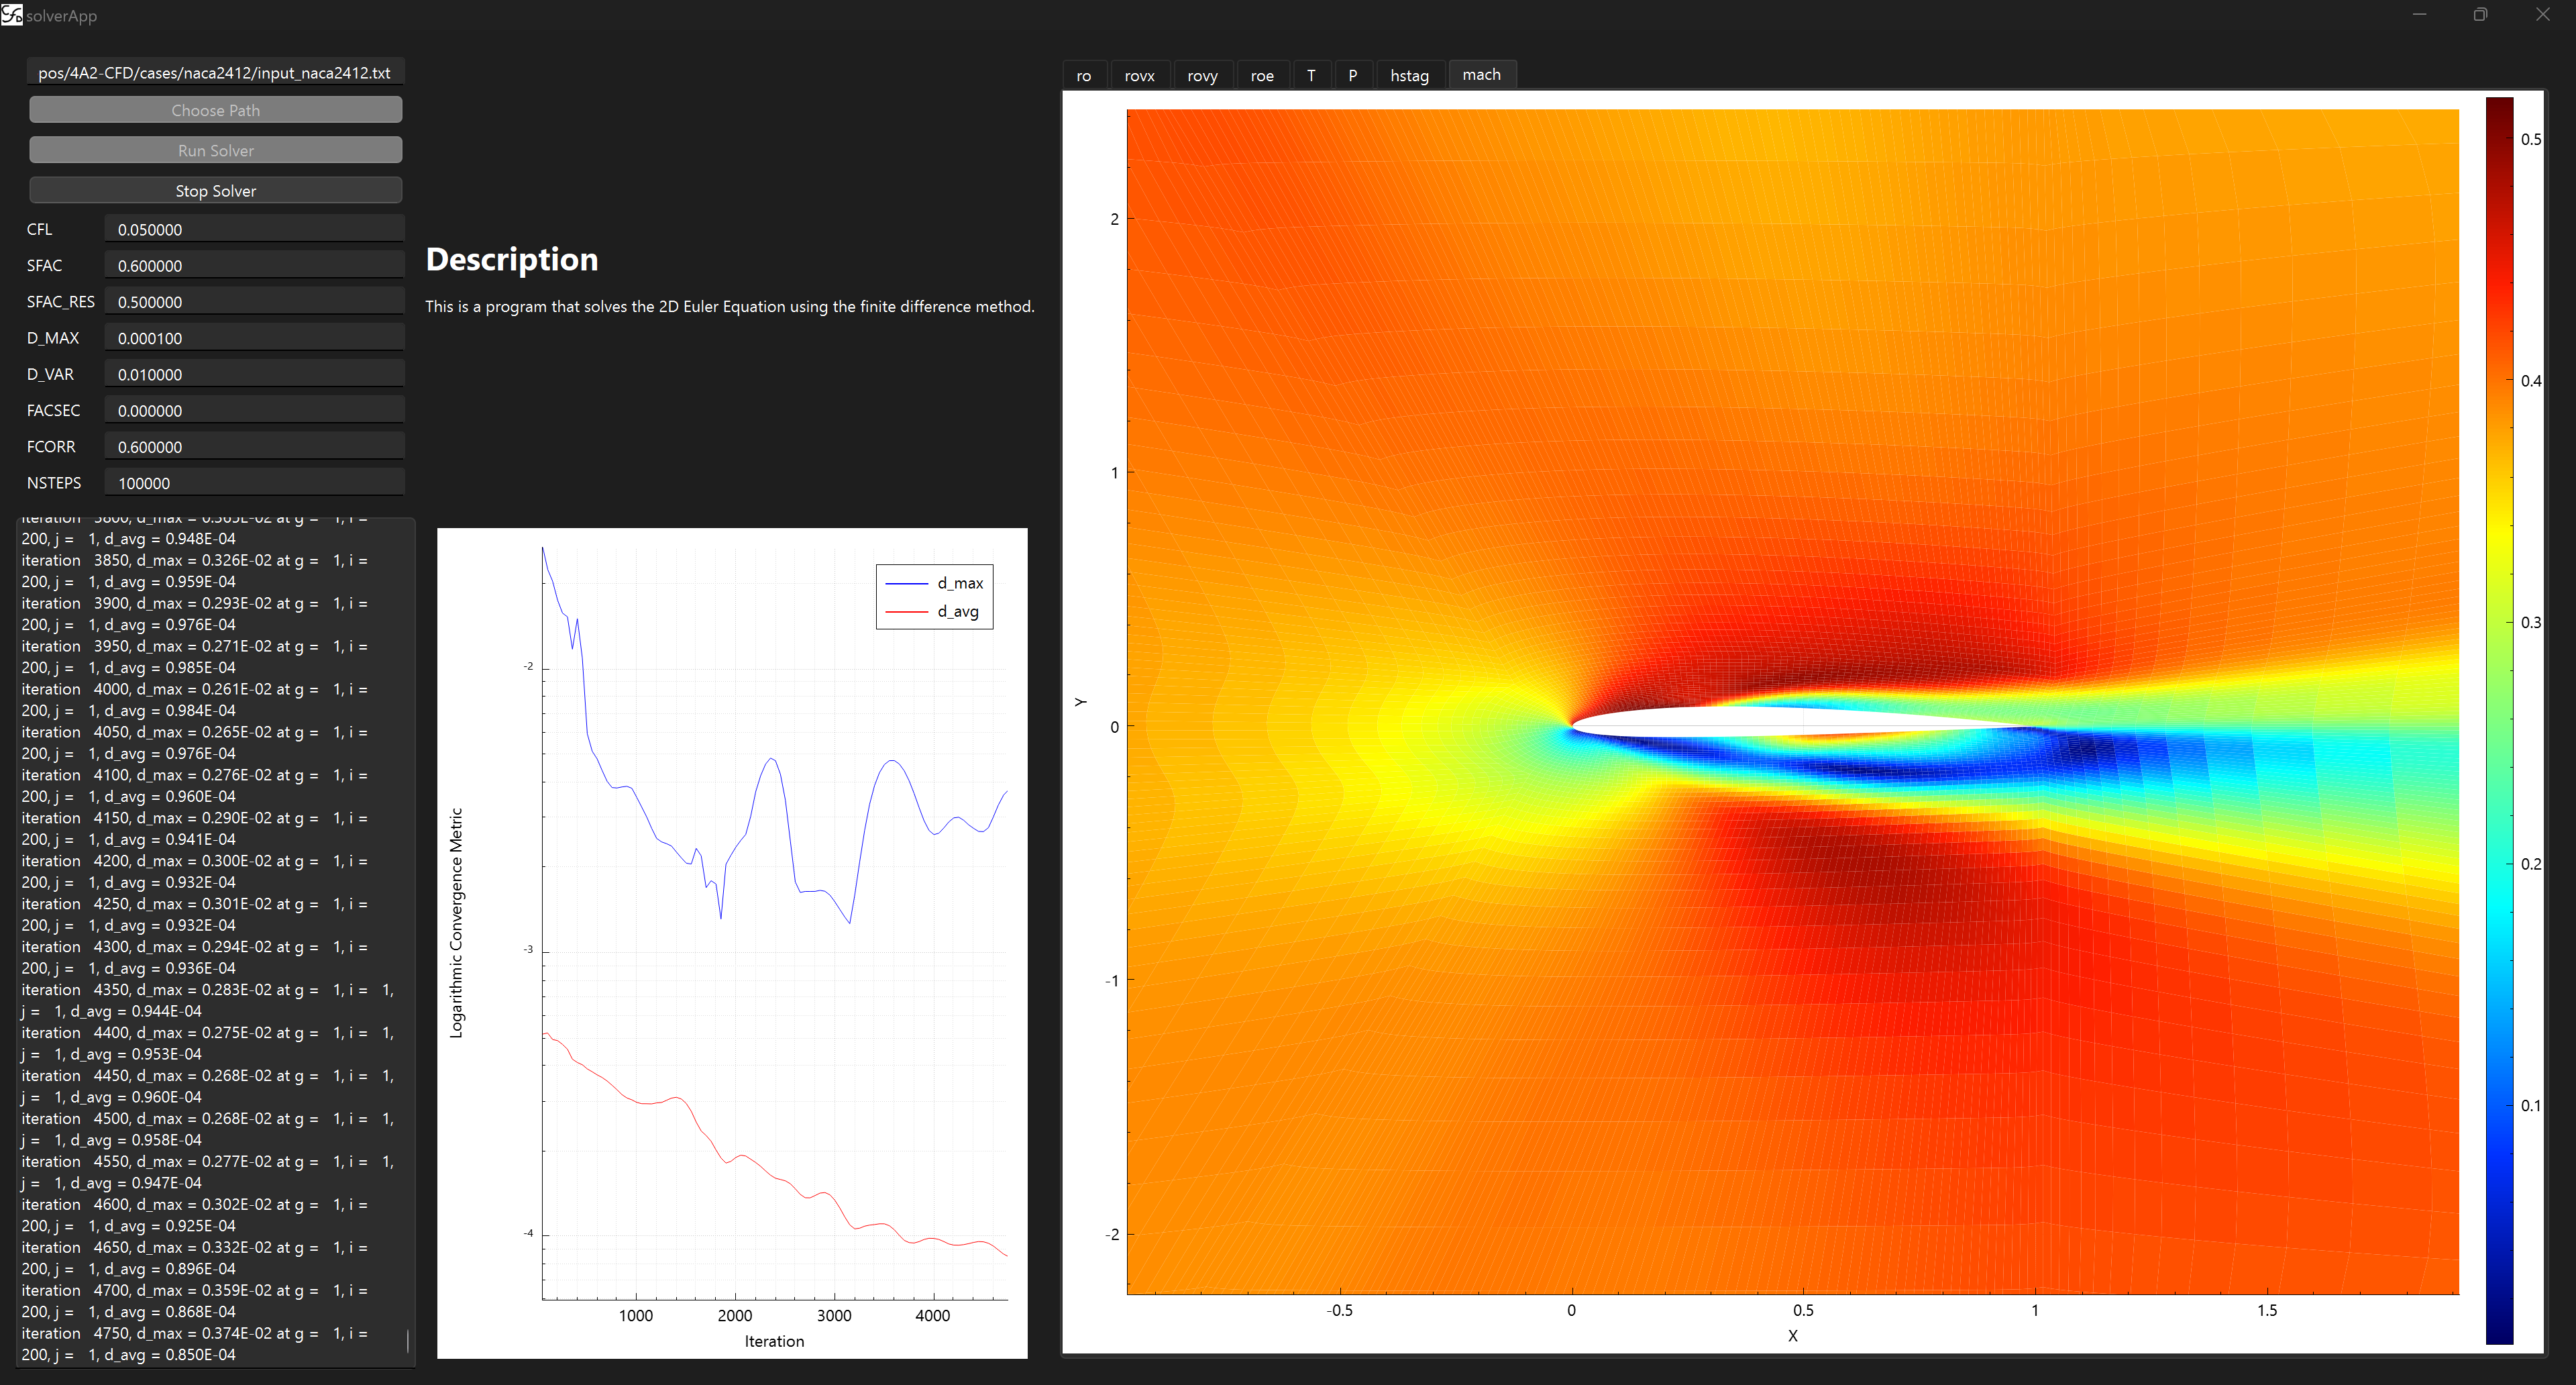
\includegraphics[width=0.7\textwidth]{figures/software.png}
    \caption{Software GUI}
    \label{fig:software}
\end{figure}

\subsection{Comparison of Improvements}

\begin{figure}[H]
    \centering
    \begin{subfigure}{0.49\textwidth}
        \centering
        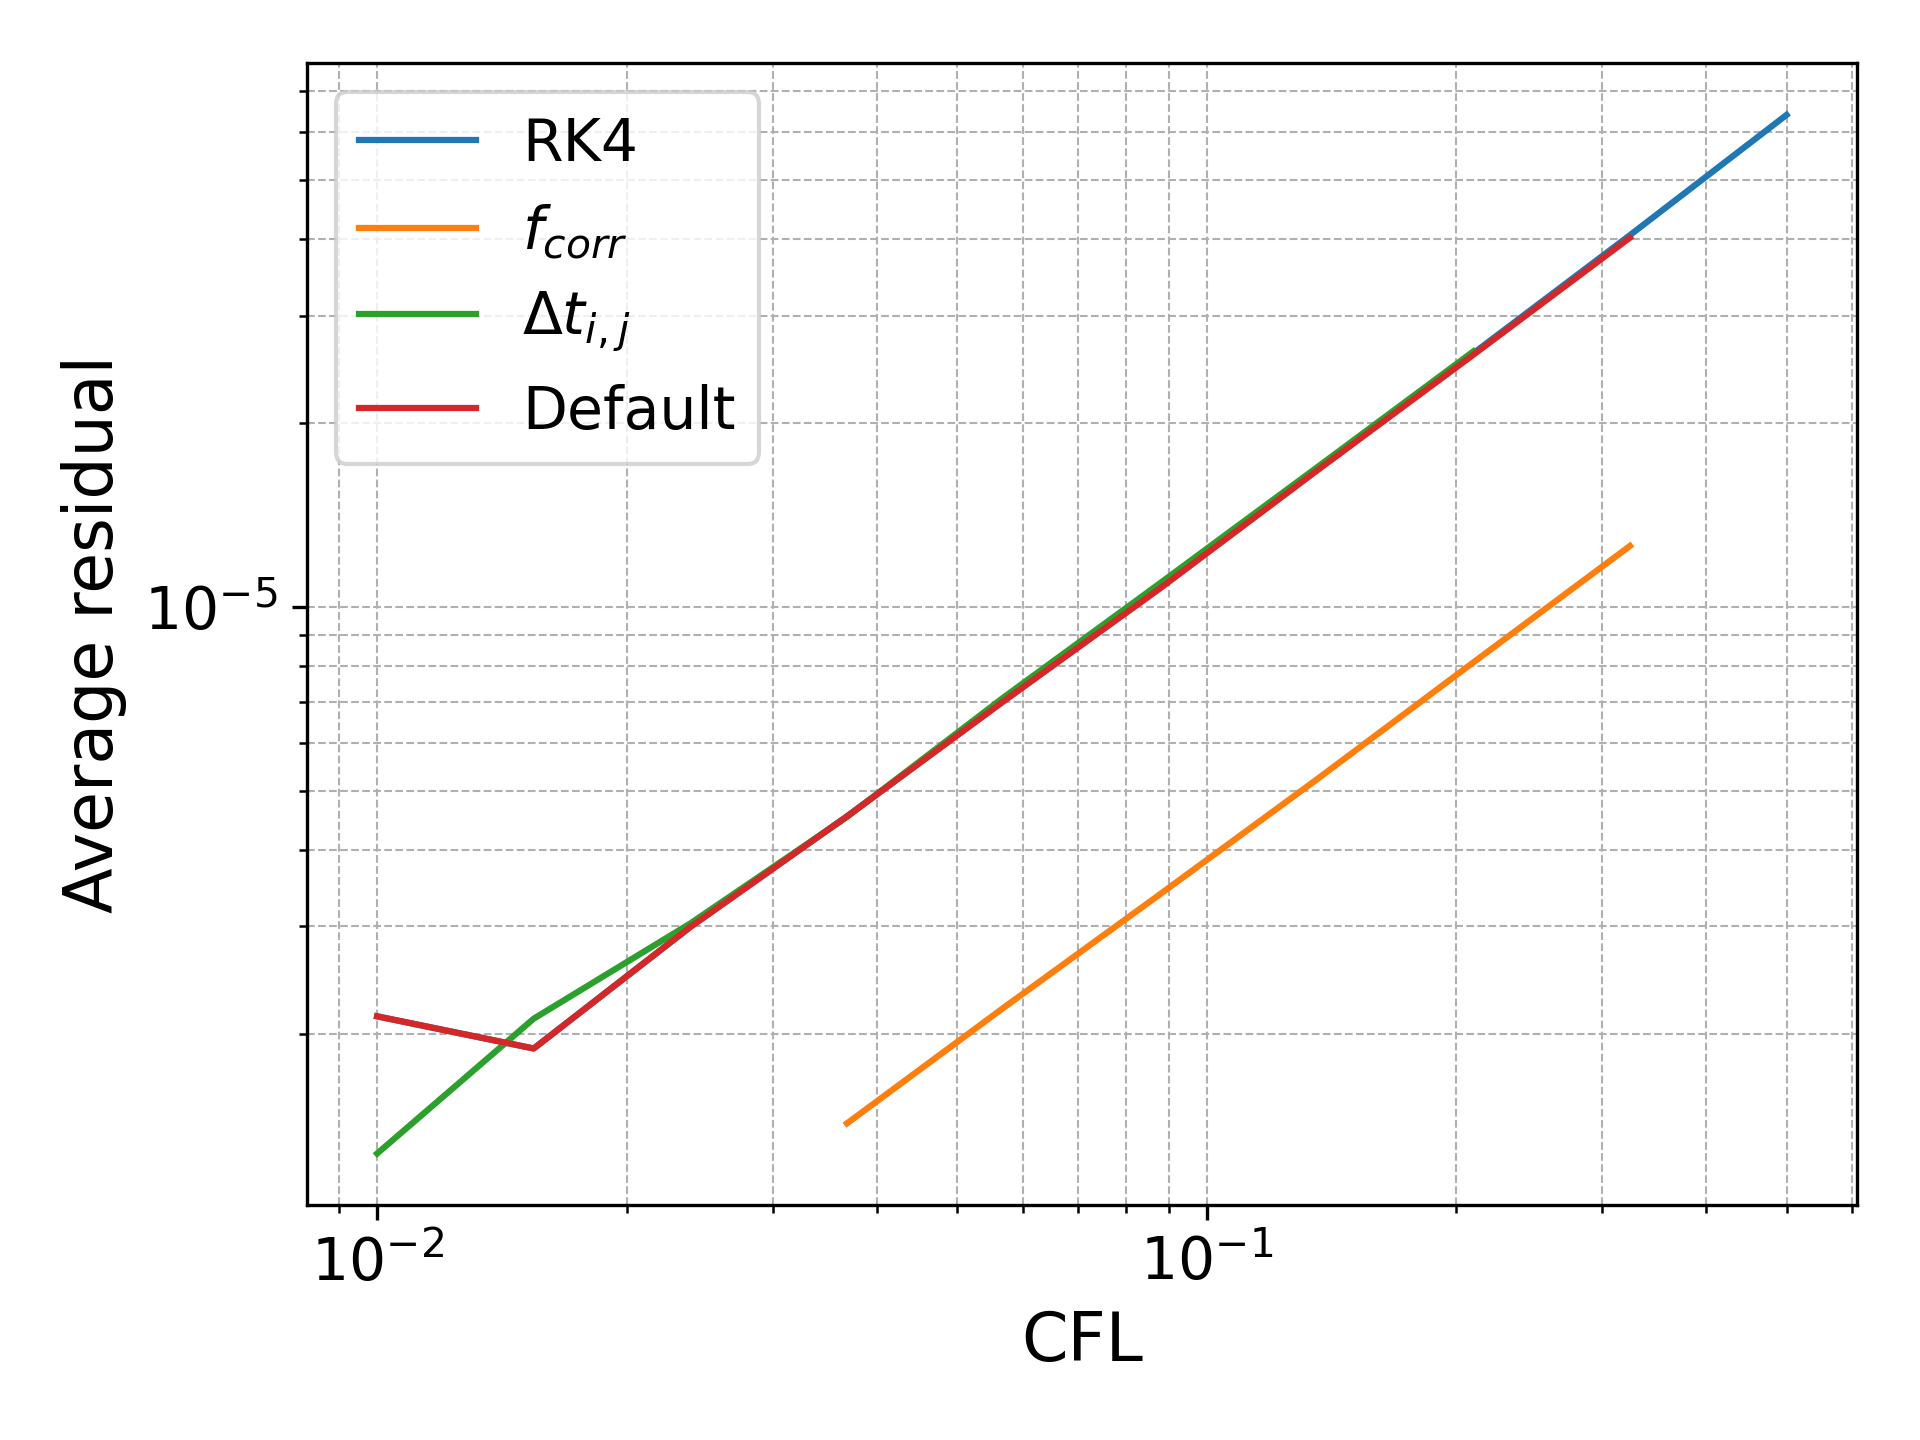
\includegraphics[width=0.99\textwidth]{figures/improvements_cfl_residual.png}
        \caption{improvements\_cfl\_residual}
        \label{fig:improvements_cfl_residual}
    \end{subfigure}
    \begin{subfigure}{0.49\textwidth}
        \centering
        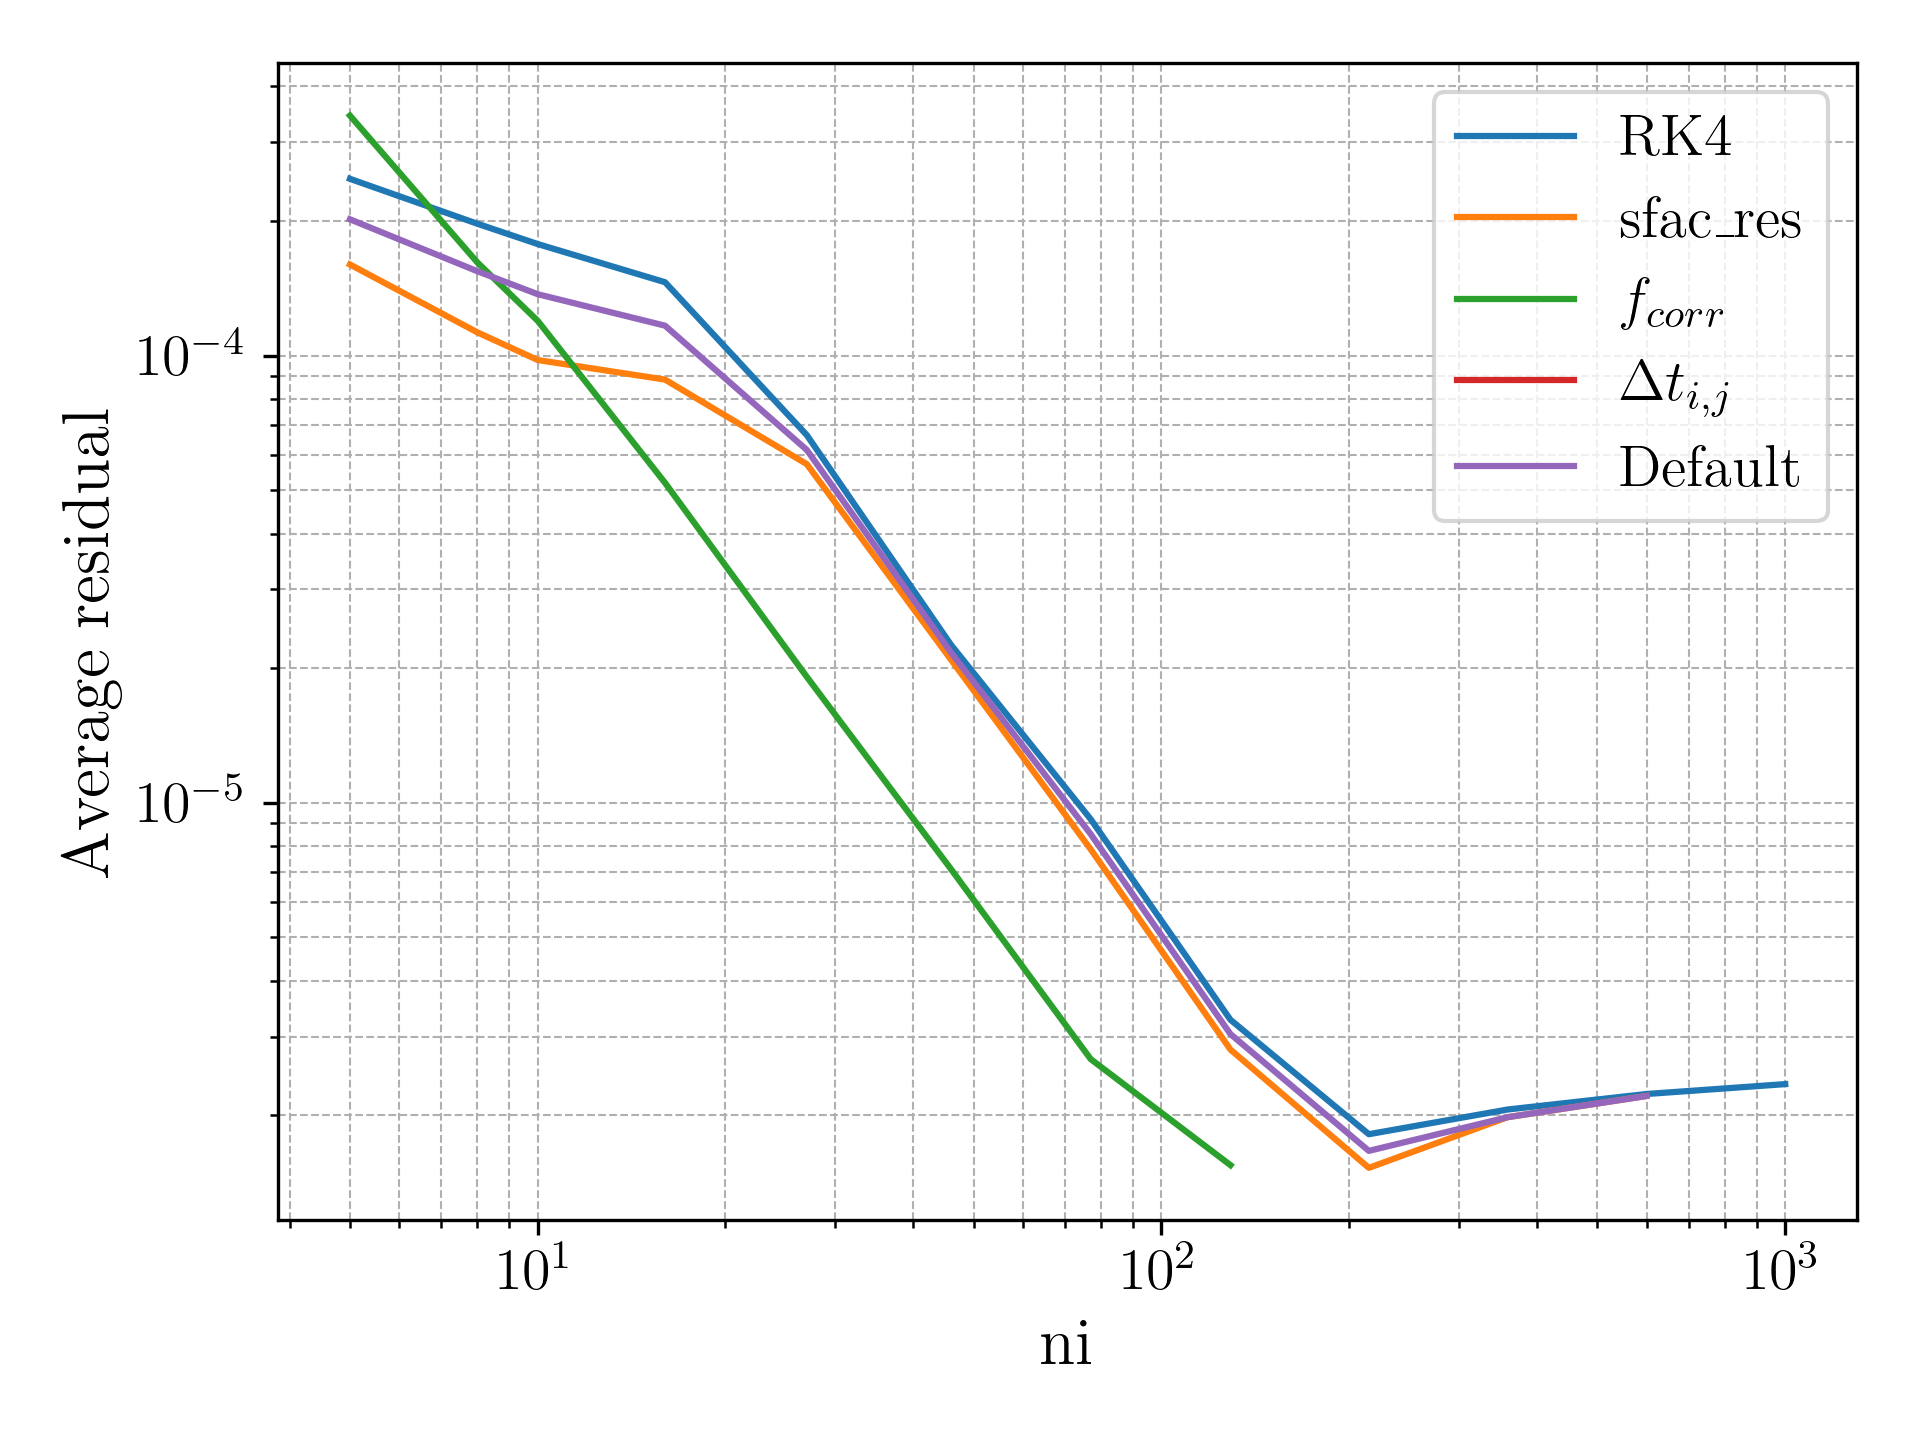
\includegraphics[width=0.99\textwidth]{figures/improvements_ni_residual.png}
        \caption{improvements\_ni\_residual}
        \label{fig:improvements_ni_residual}
    \end{subfigure}
    \caption{Comparison of improvements}
\end{figure}

\begin{figure}[H]
    \centering
    \begin{subfigure}{0.49\textwidth}
        \centering
        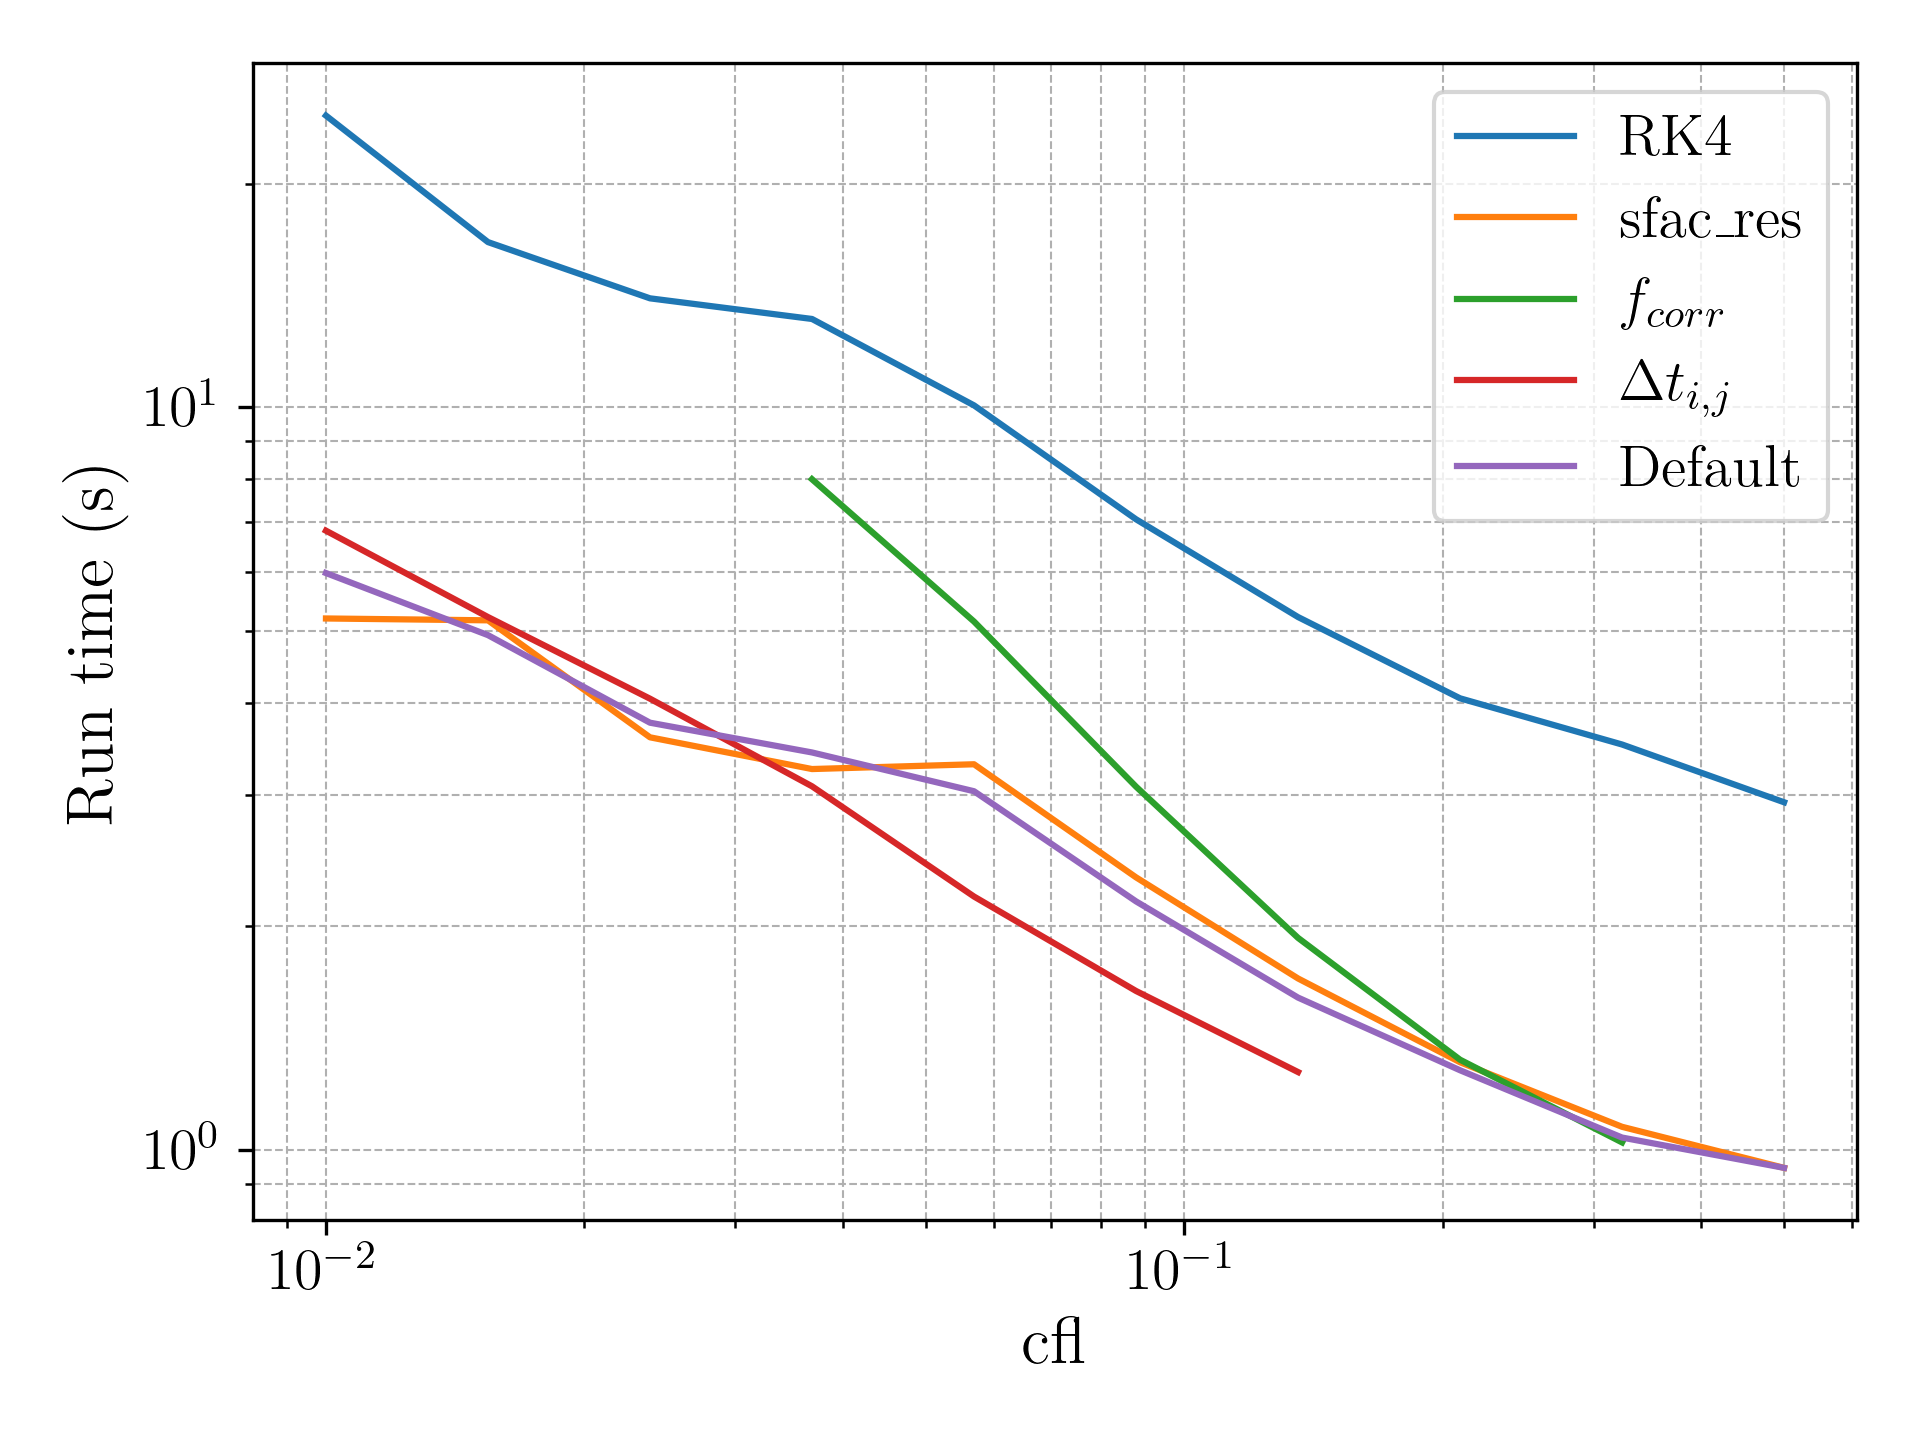
\includegraphics[width=0.99\textwidth]{figures/improvements_cfl_time.png}
        \caption{improvements\_cfl\_time}
        \label{fig:improvements_cfl_time}
    \end{subfigure}
    \begin{subfigure}{0.49\textwidth}
        \centering
        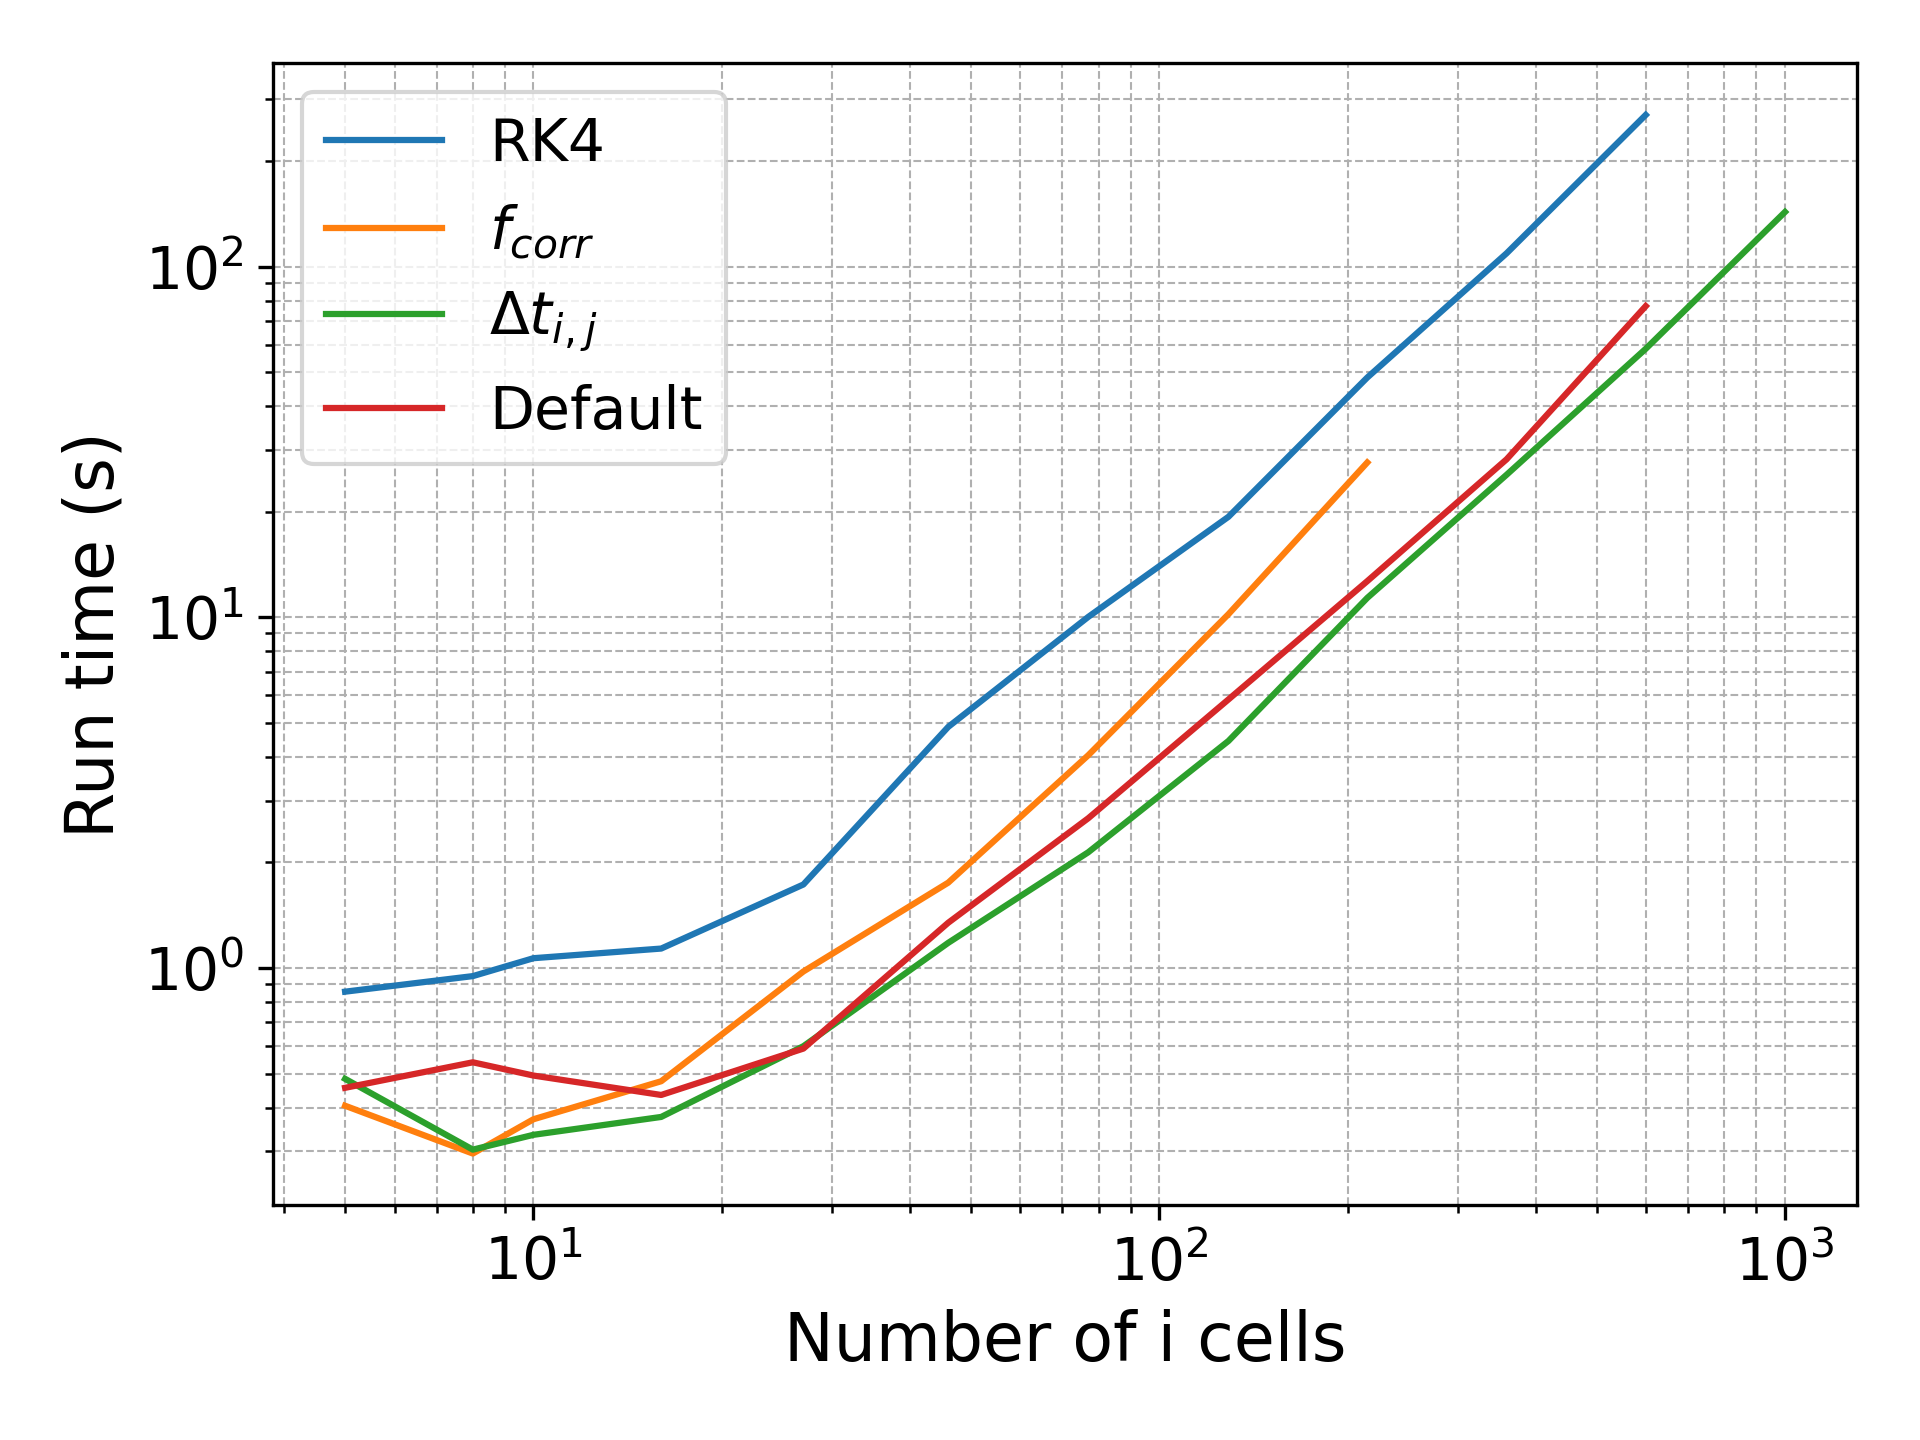
\includegraphics[width=0.99\textwidth]{figures/improvements_ni_time.png}
        \caption{improvements\_ni\_time}
        \label{fig:improvements_ni_time}
    \end{subfigure}
    \caption{Comparison of improvements}
\end{figure}


\subsection{Naca airfoils}

\begin{figure}[H]
    \centering
    \begin{subfigure}{0.49\textwidth}
        \centering
        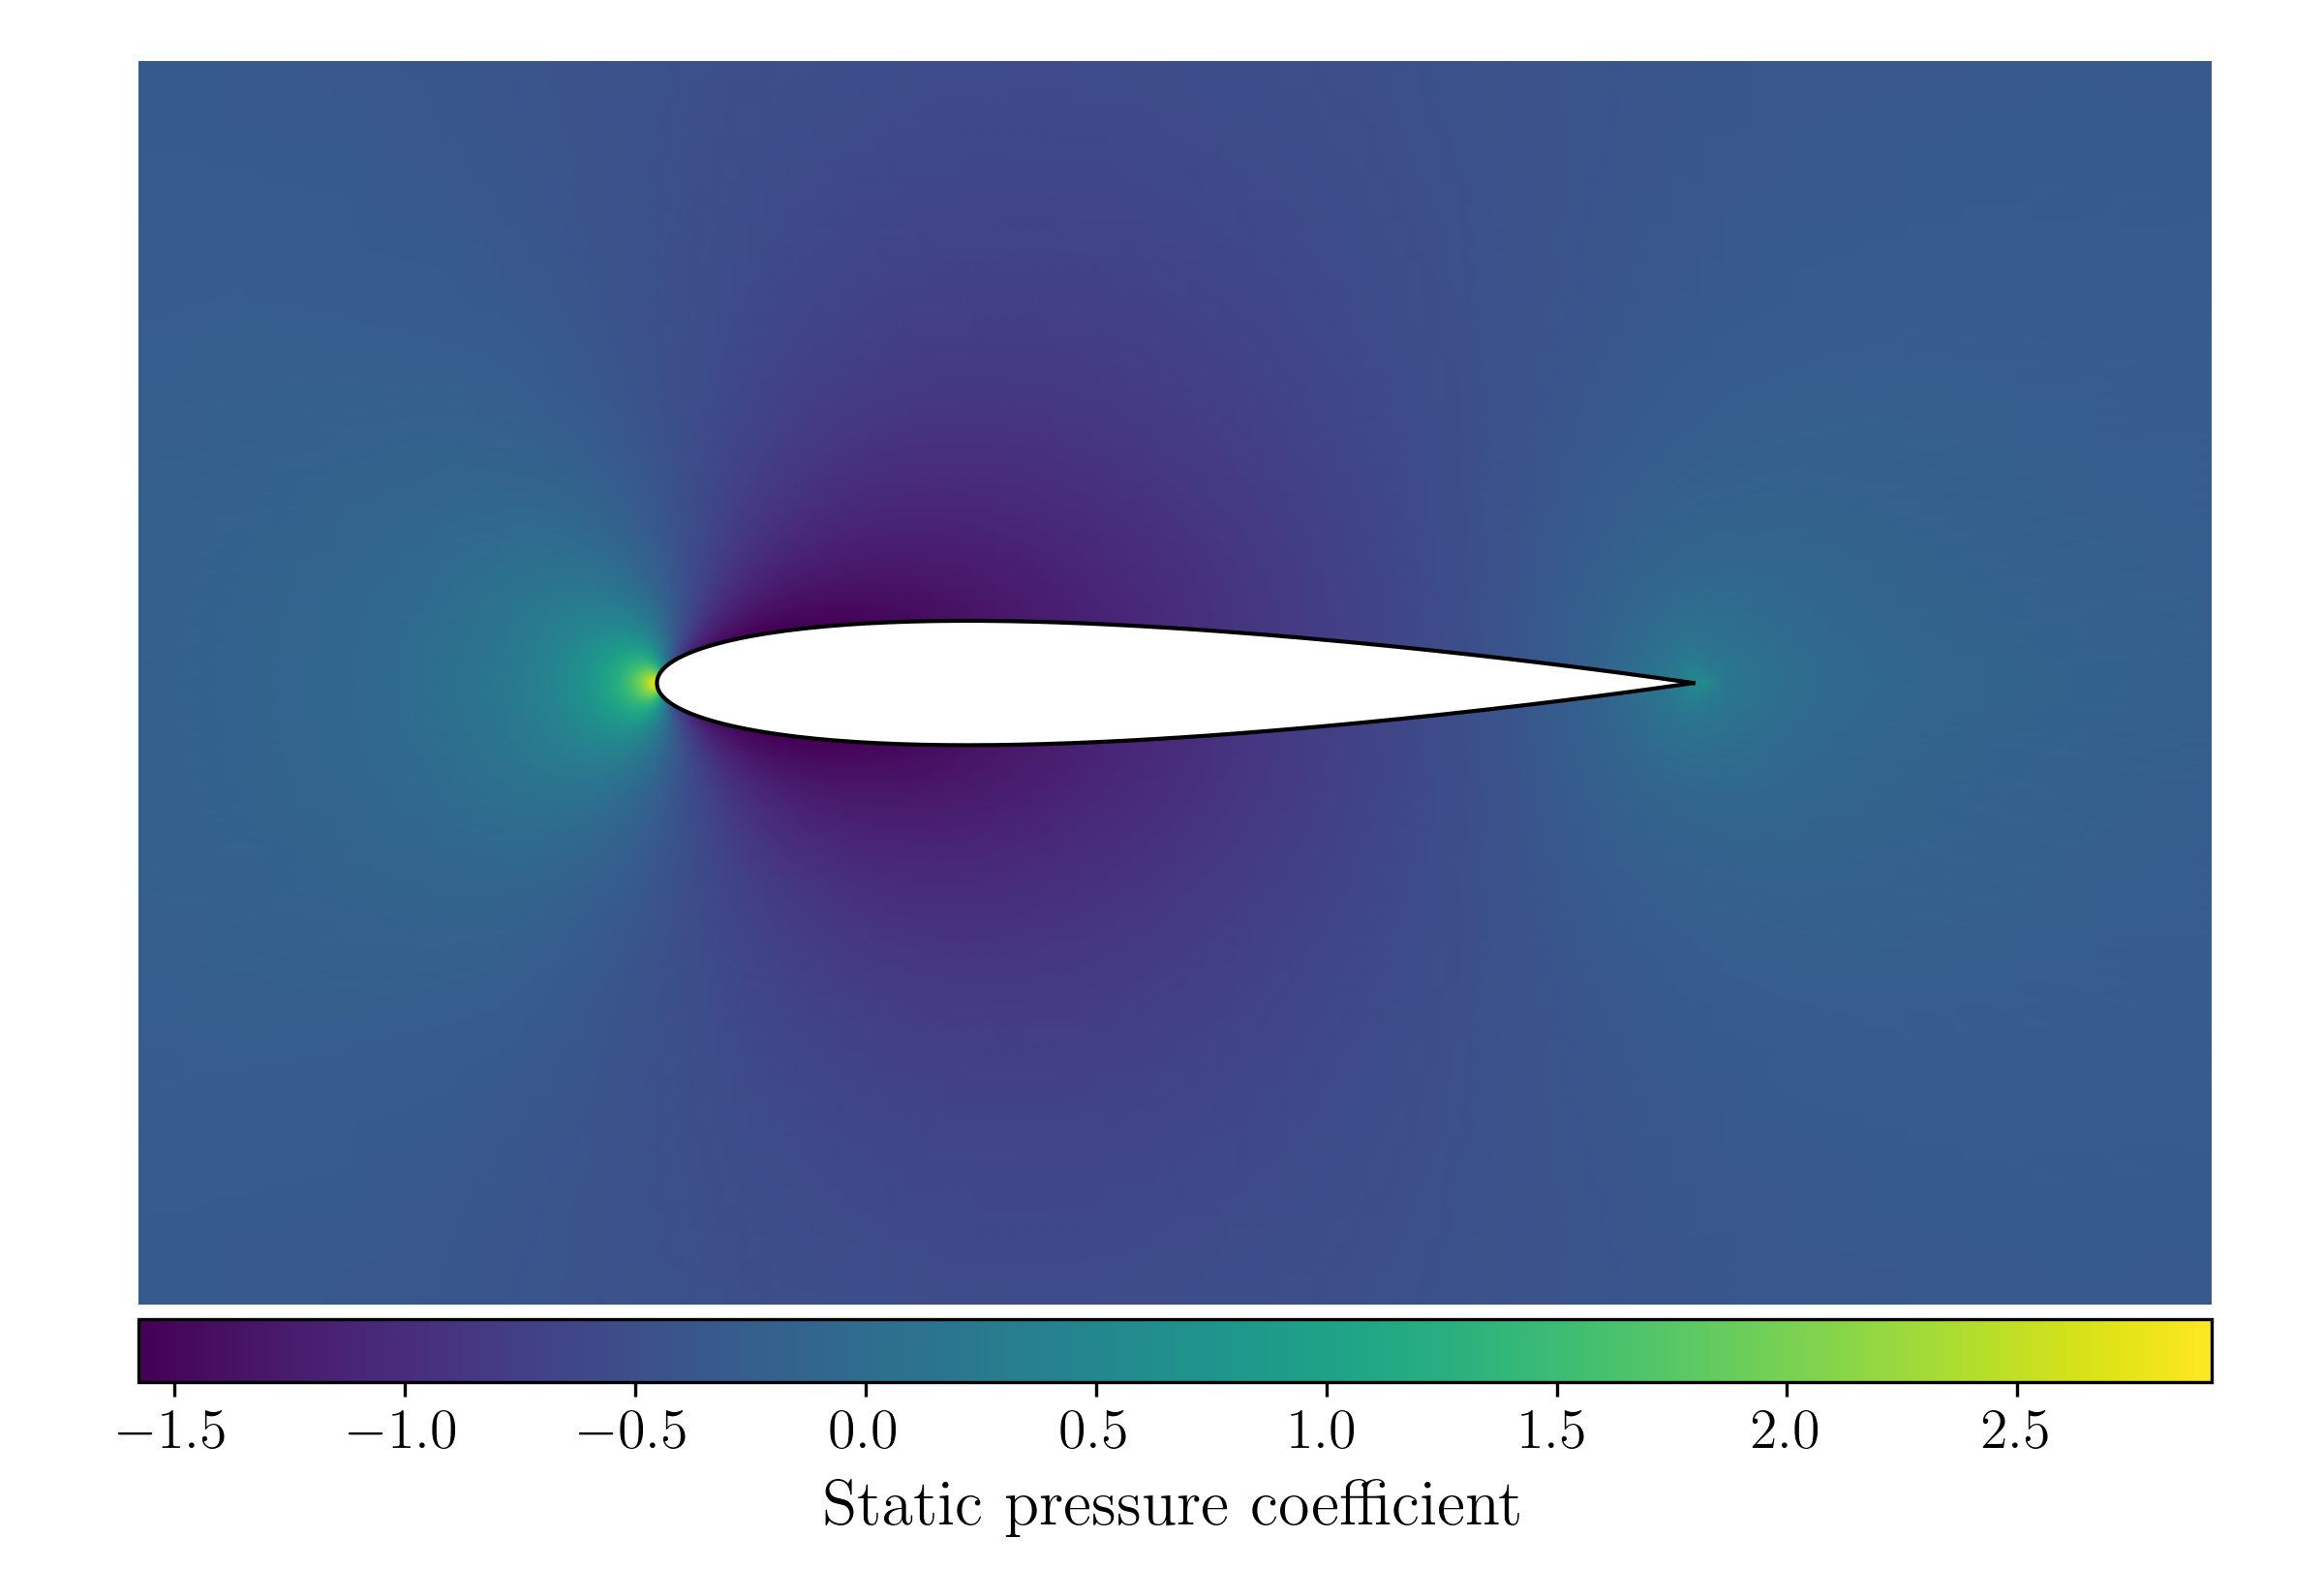
\includegraphics[width=0.99\textwidth]{figures/naca0012_cp.png}
        \caption{}
        \label{fig:naca0012_cp}
    \end{subfigure}
    \begin{subfigure}{0.49\textwidth}
        \centering
        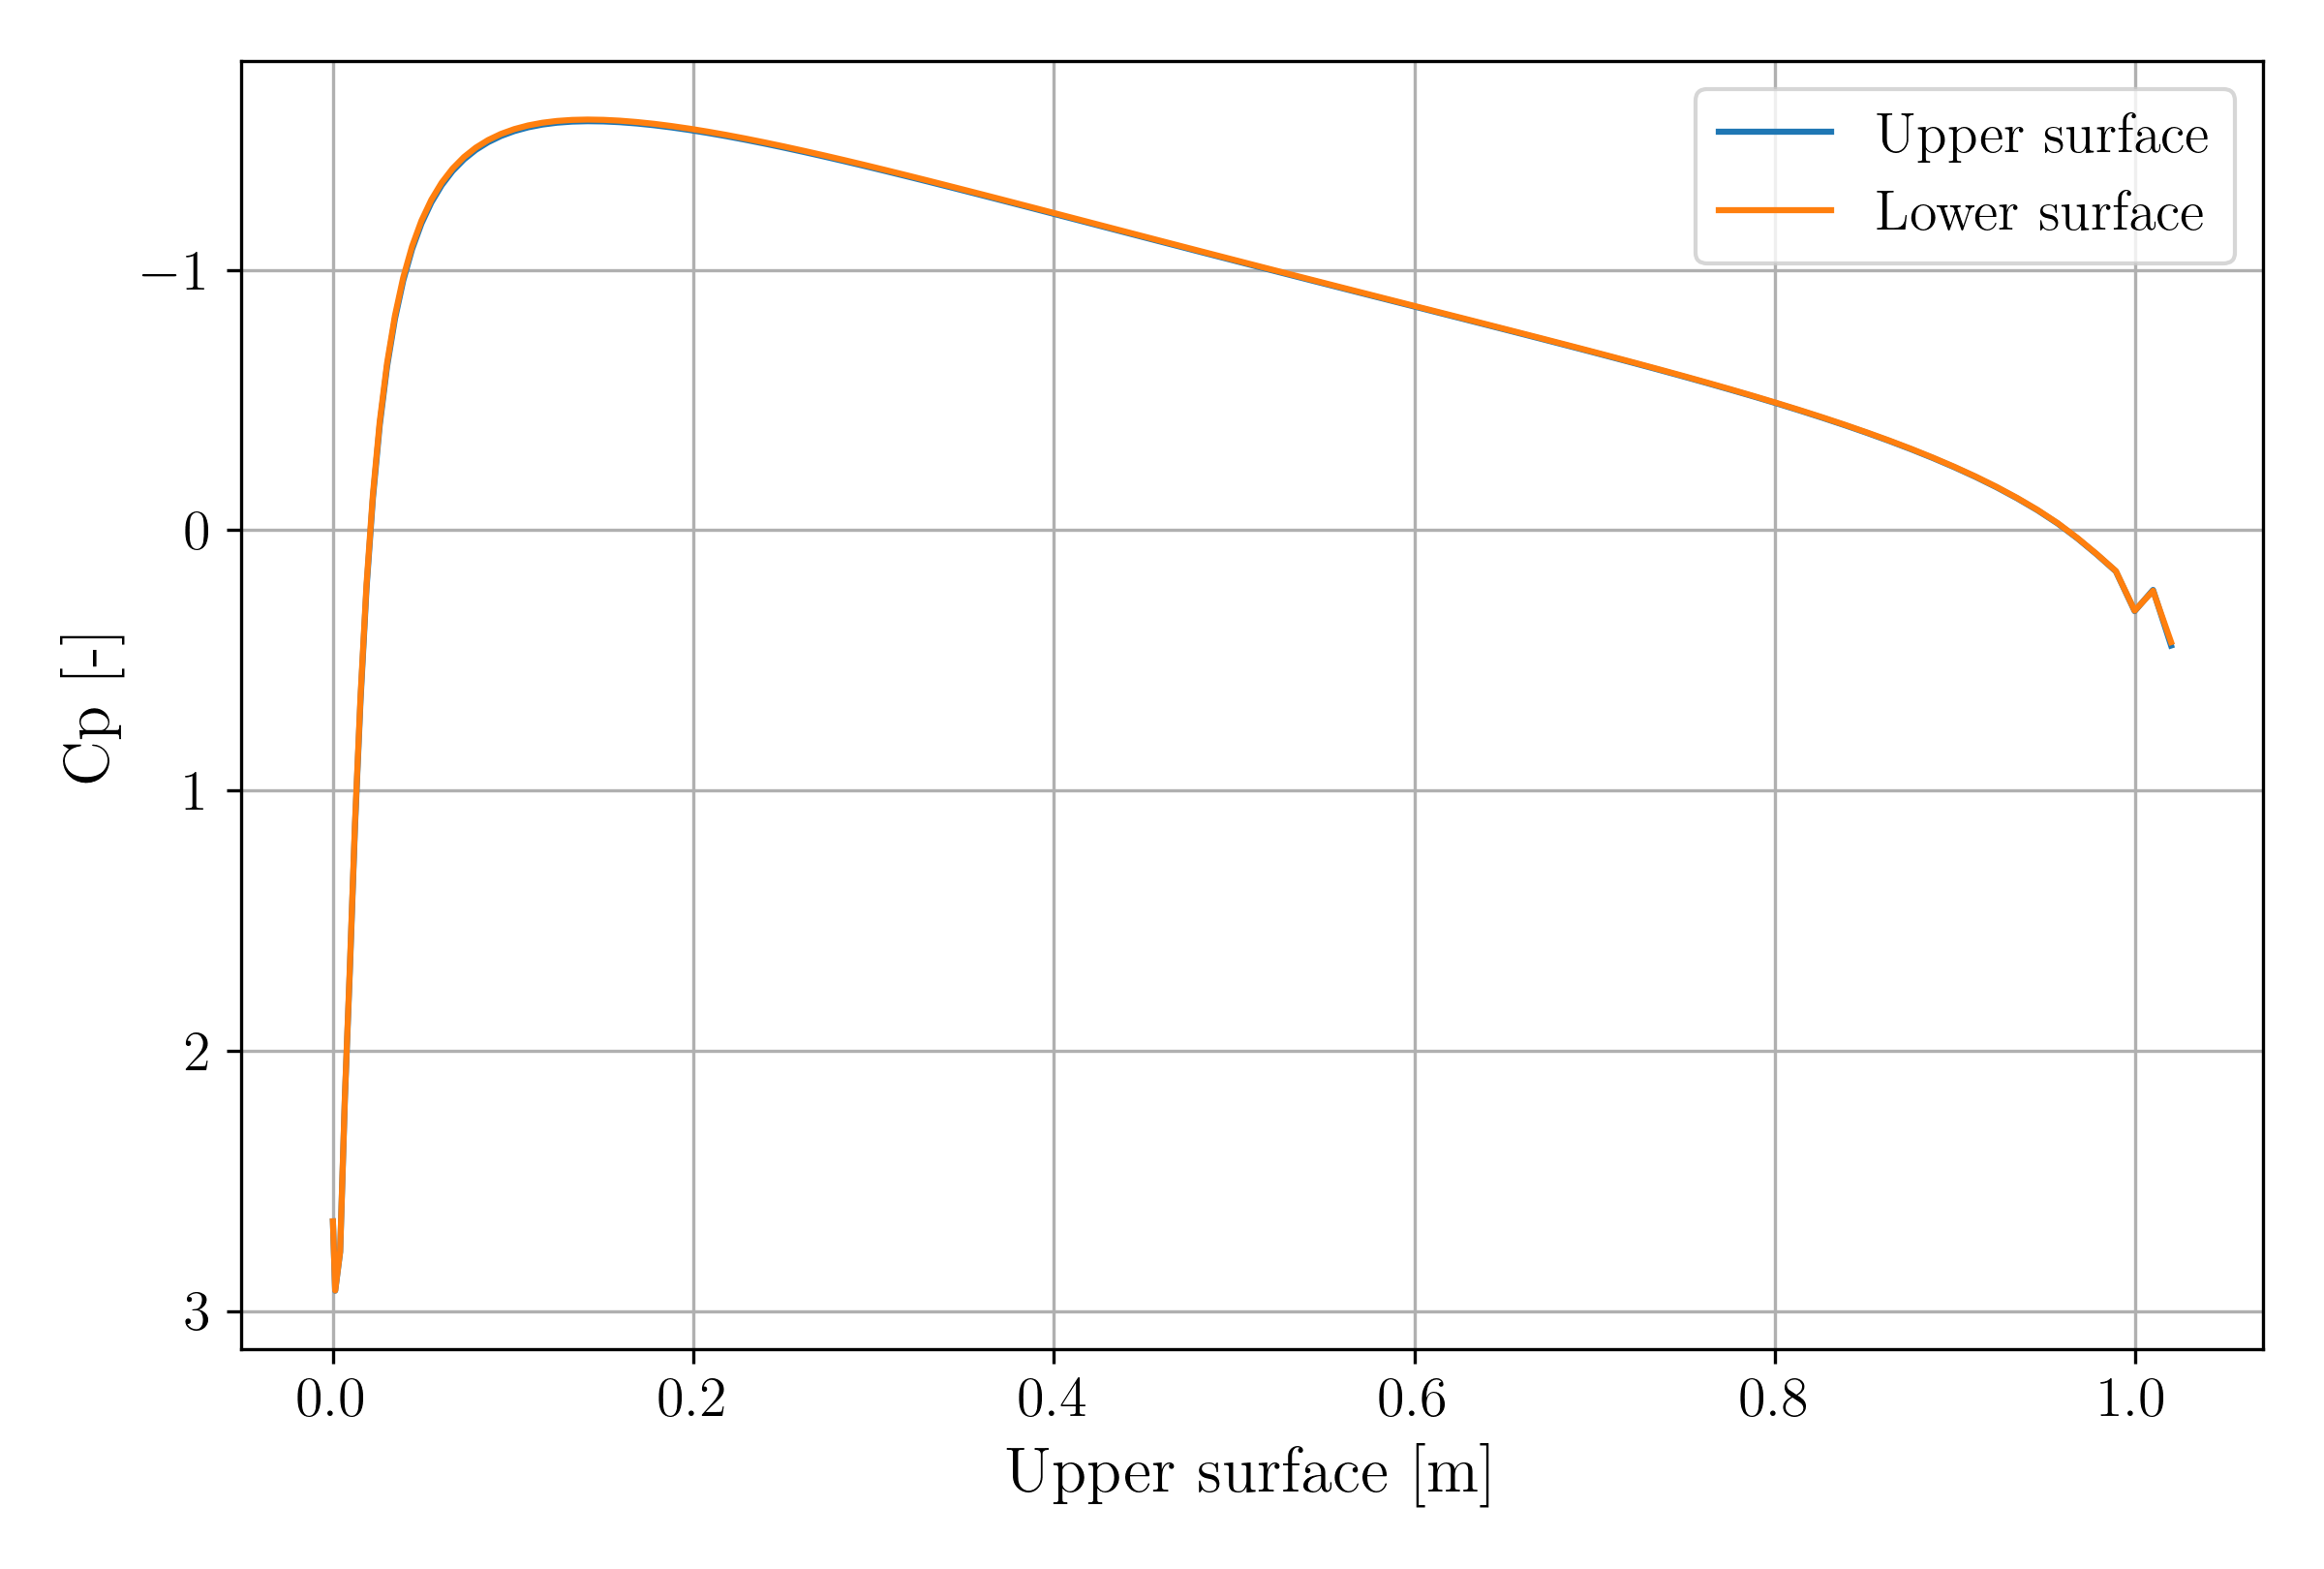
\includegraphics[width=0.99\textwidth]{figures/naca0012_surface_cp.png}
        \caption{}
        \label{fig:naca0012_mach}
    \end{subfigure}
    \caption{Naca0012 test case results}
\end{figure}

\begin{figure}[H]
    \centering
    \begin{subfigure}{0.49\textwidth}
        \centering
        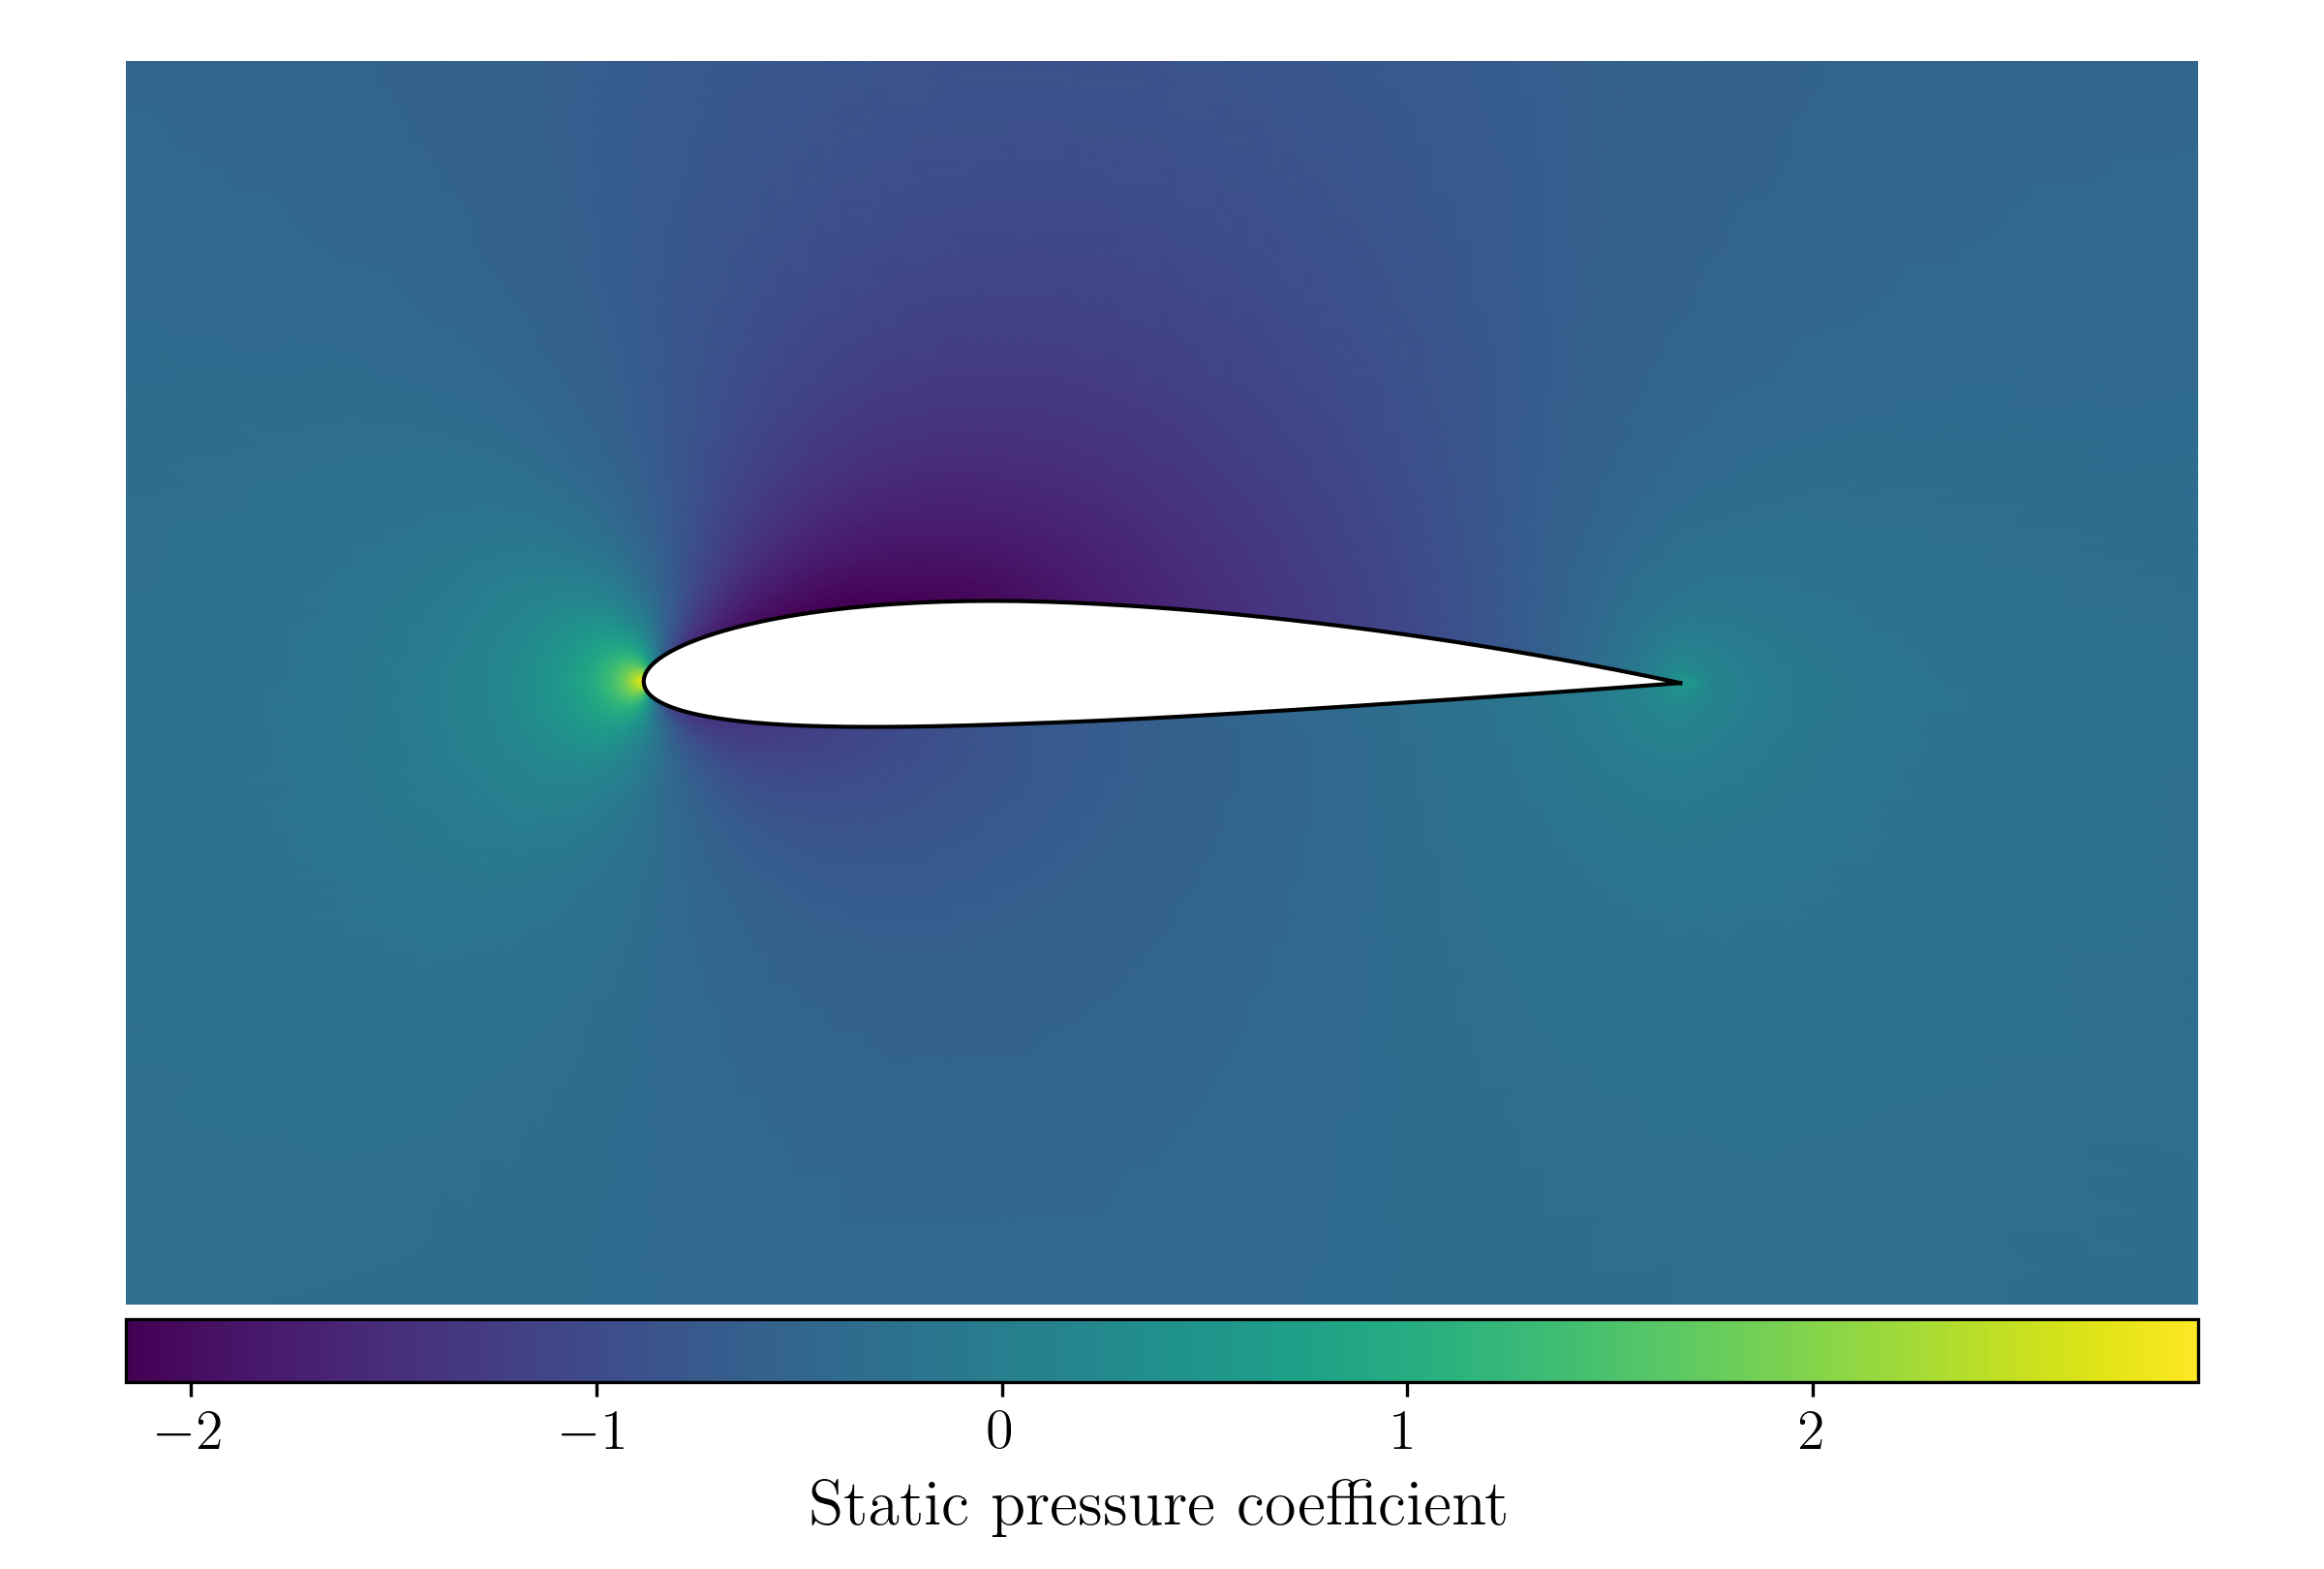
\includegraphics[width=0.99\textwidth]{figures/naca2412_cp.png}
        \caption{}
        \label{fig:naca2412_cp}
    \end{subfigure}
    \begin{subfigure}{0.49\textwidth}
        \centering
        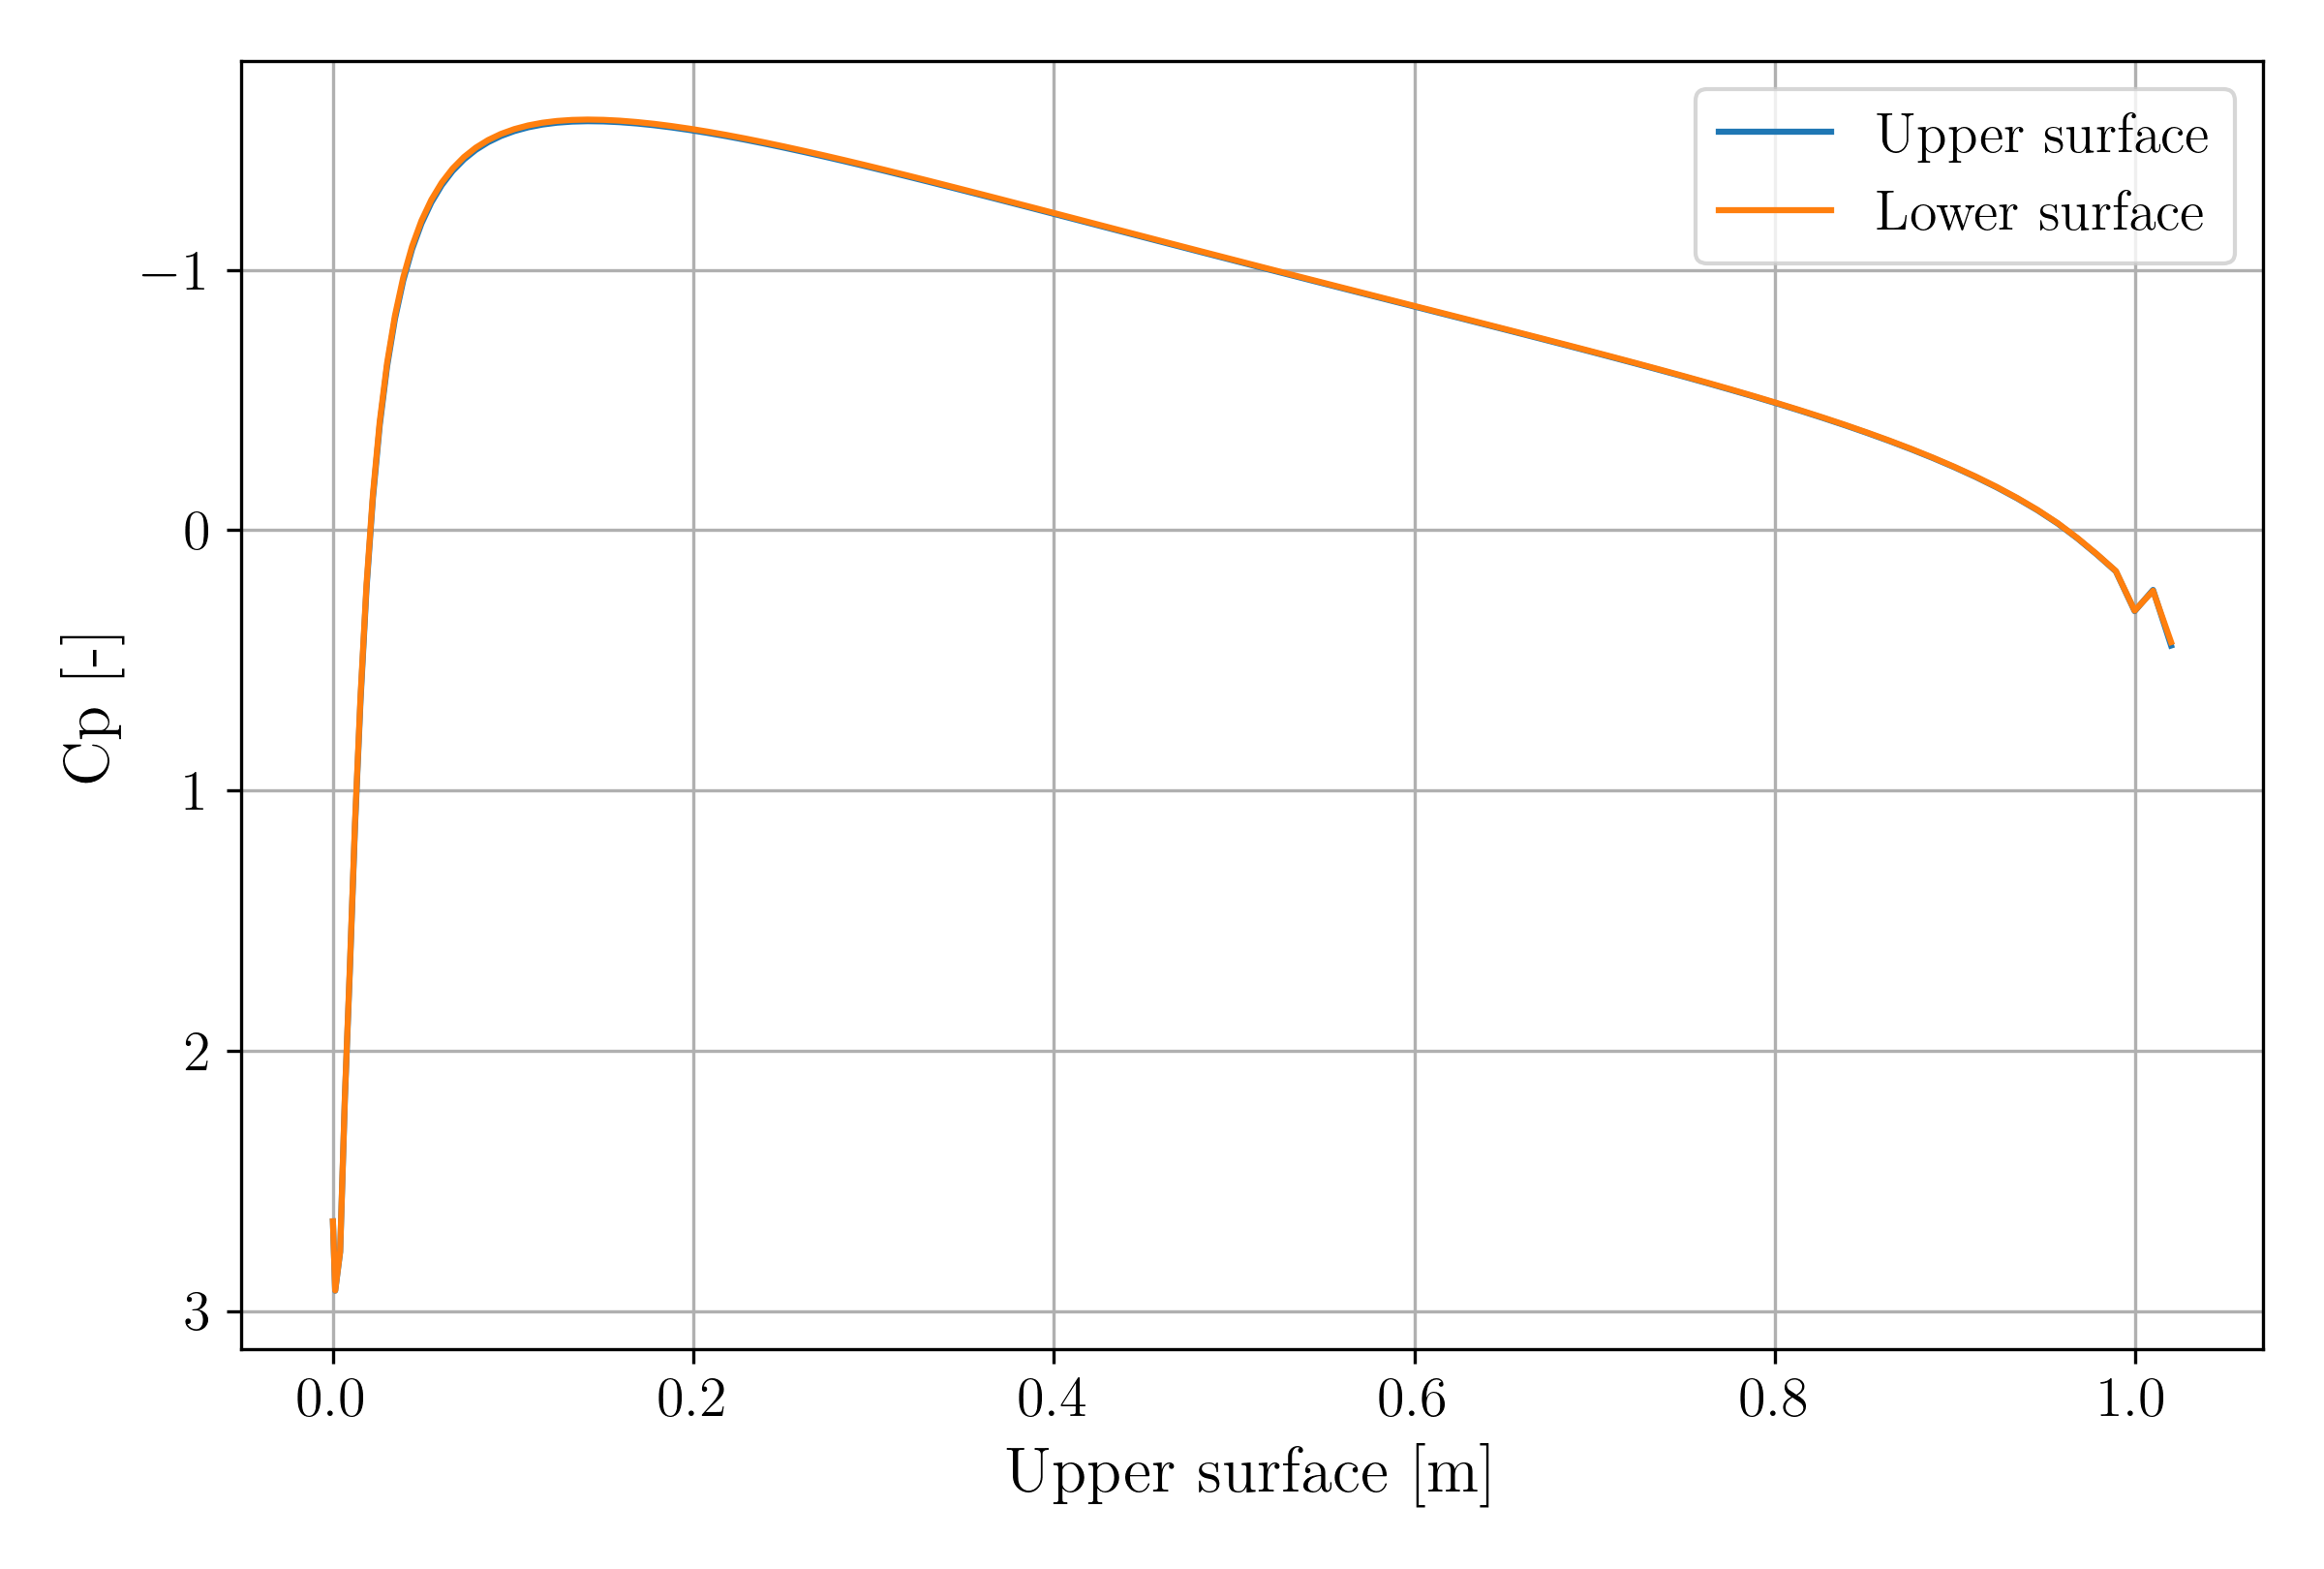
\includegraphics[width=0.99\textwidth]{figures/naca0012_surface_cp.png}
        \caption{}
        \label{fig:naca2412_mach}
    \end{subfigure}
    \caption{Naca2412 test case results}
\end{figure}

\begin{figure}[H]
    \centering
    \begin{subfigure}{0.49\textwidth}
        \centering
        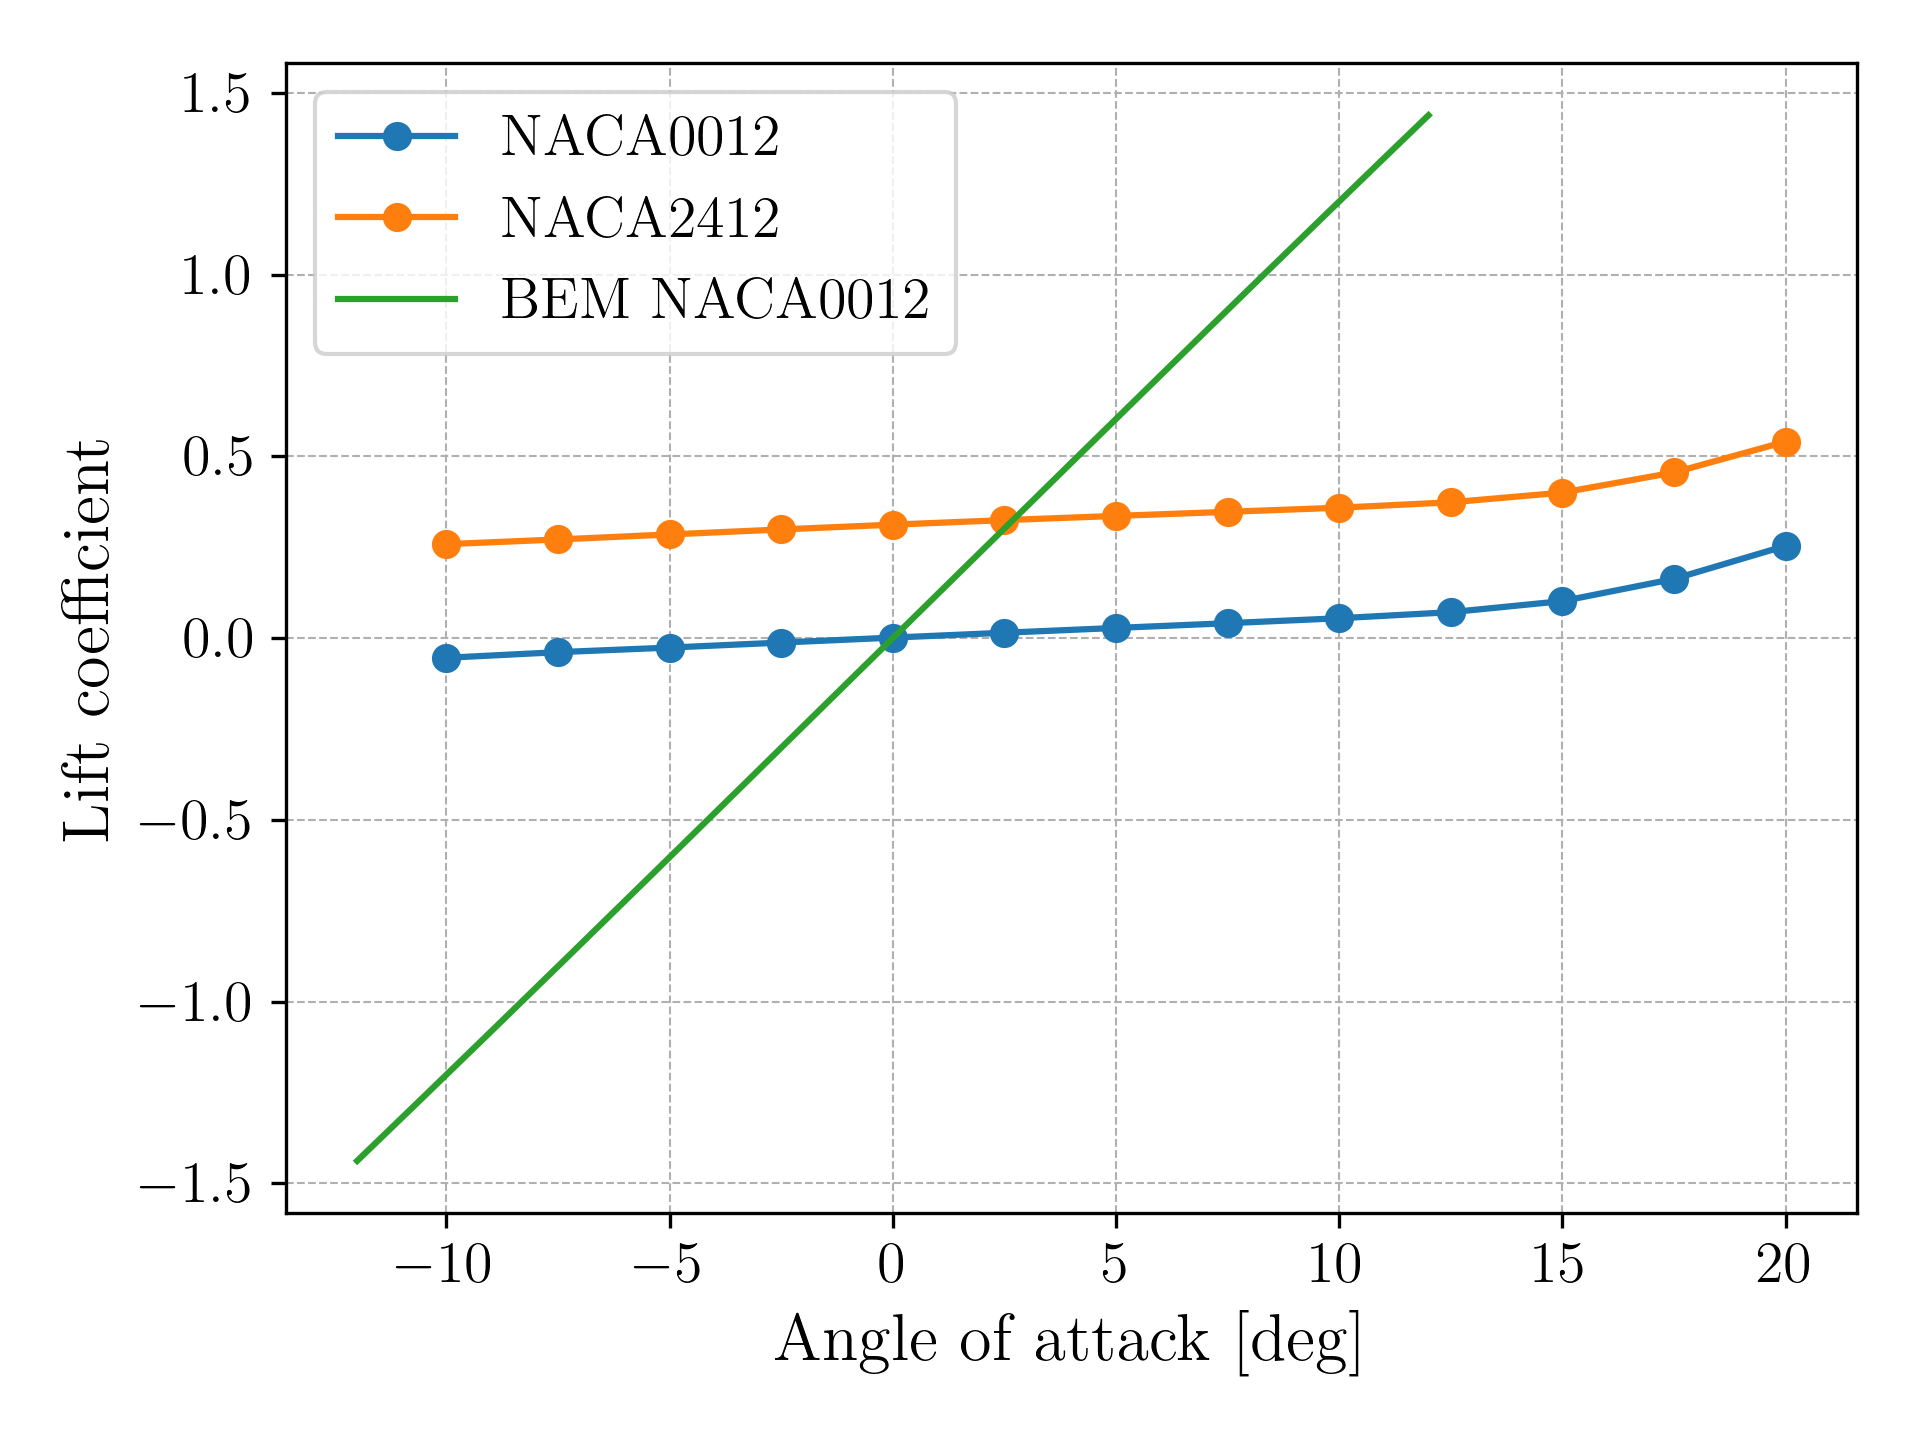
\includegraphics[width=0.99\textwidth]{figures/cl_alpha.png}
        \caption{}
        \label{fig:cl_alpha}
    \end{subfigure}
    \begin{subfigure}{0.49\textwidth}
        \centering
        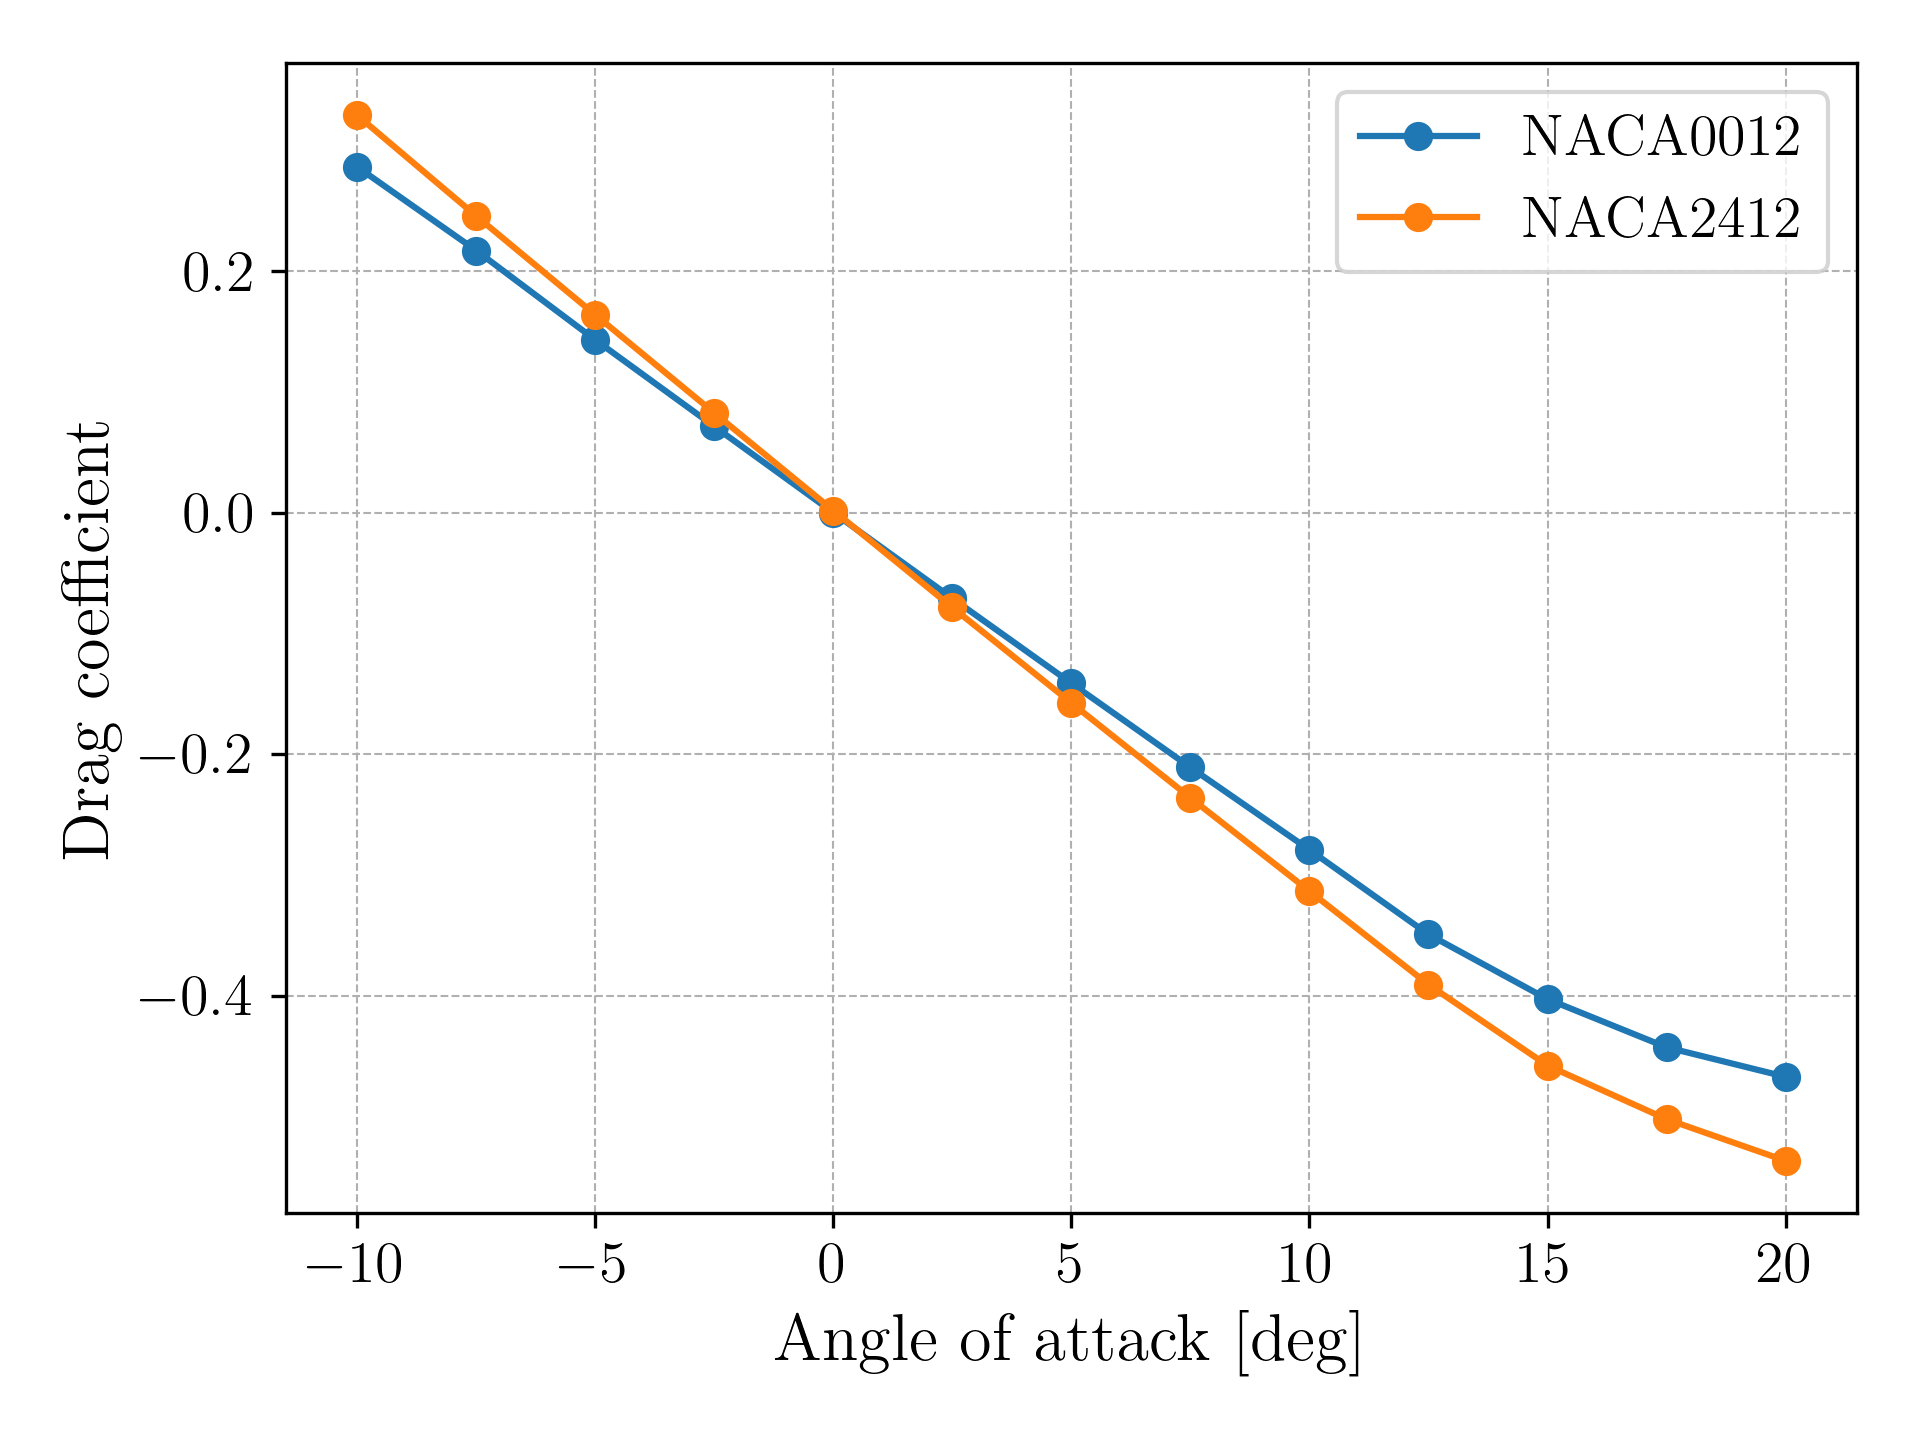
\includegraphics[width=0.99\textwidth]{figures/cd_alpha.png}
        \caption{}
        \label{fig:cd_alpha}
    \end{subfigure}
    \caption{Naca2412 test case results}
\end{figure}

\subsection{Turbine}

\begin{figure}[H]
    \centering
    \begin{subfigure}{0.49\textwidth}
        \centering
        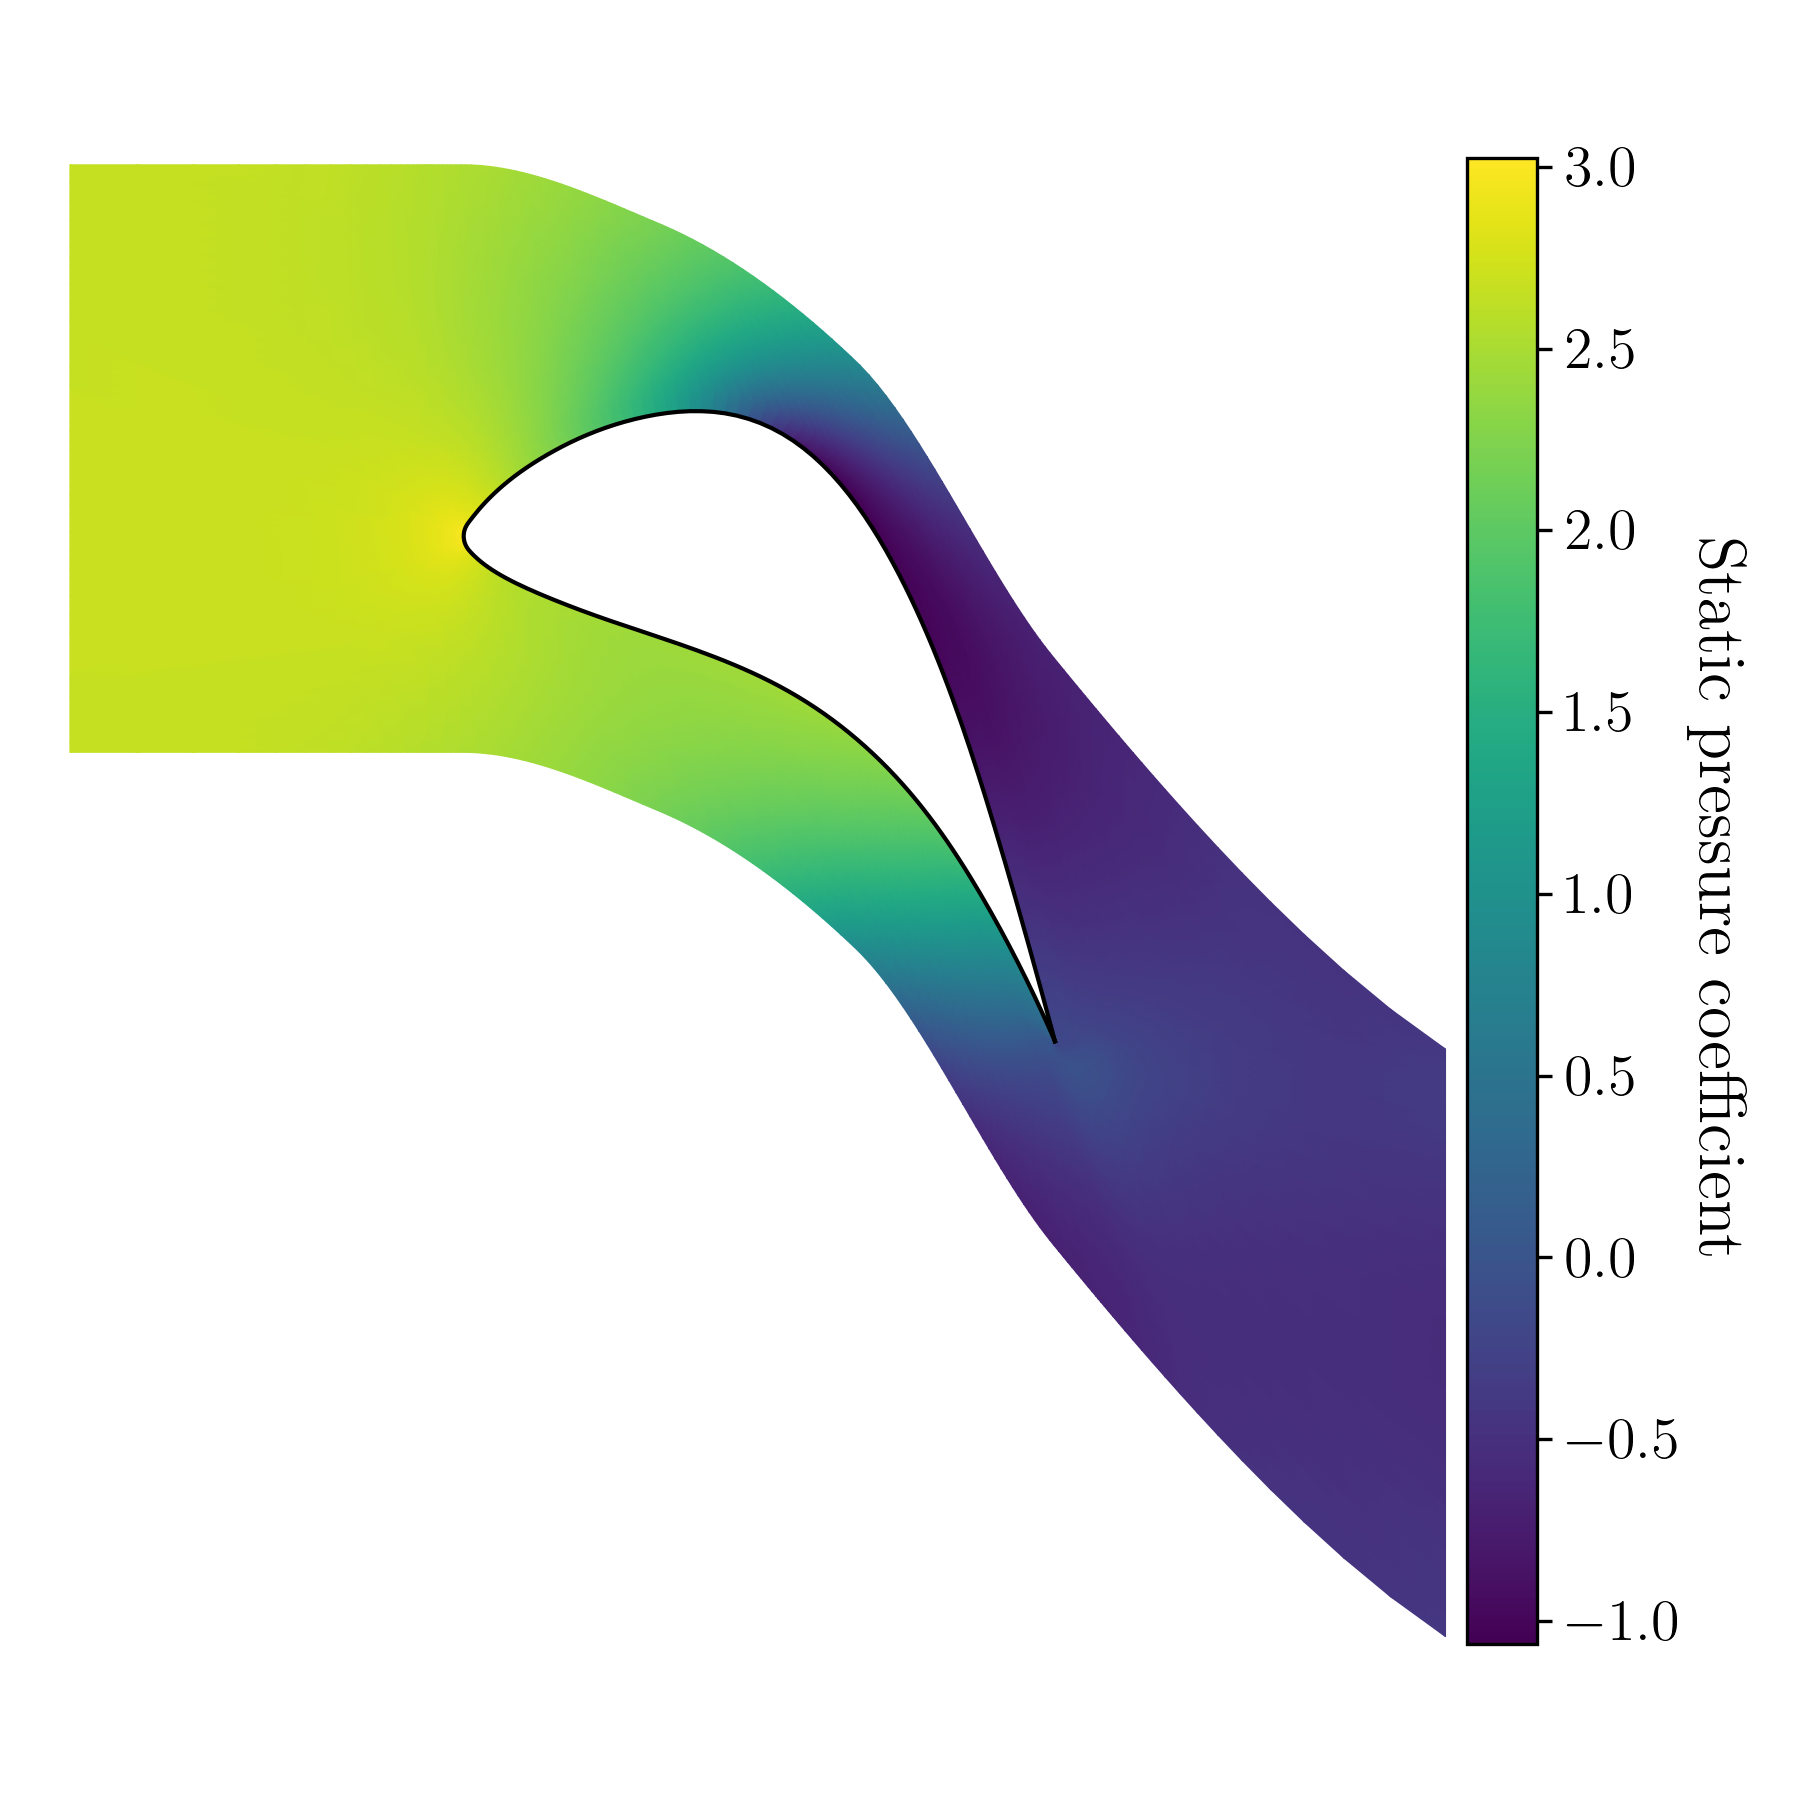
\includegraphics[width=0.99\textwidth]{figures/turbine_c_cp.png}
        \caption{}
        \label{fig:turbine_c_cp}
    \end{subfigure}
    \begin{subfigure}{0.49\textwidth}
        \centering
        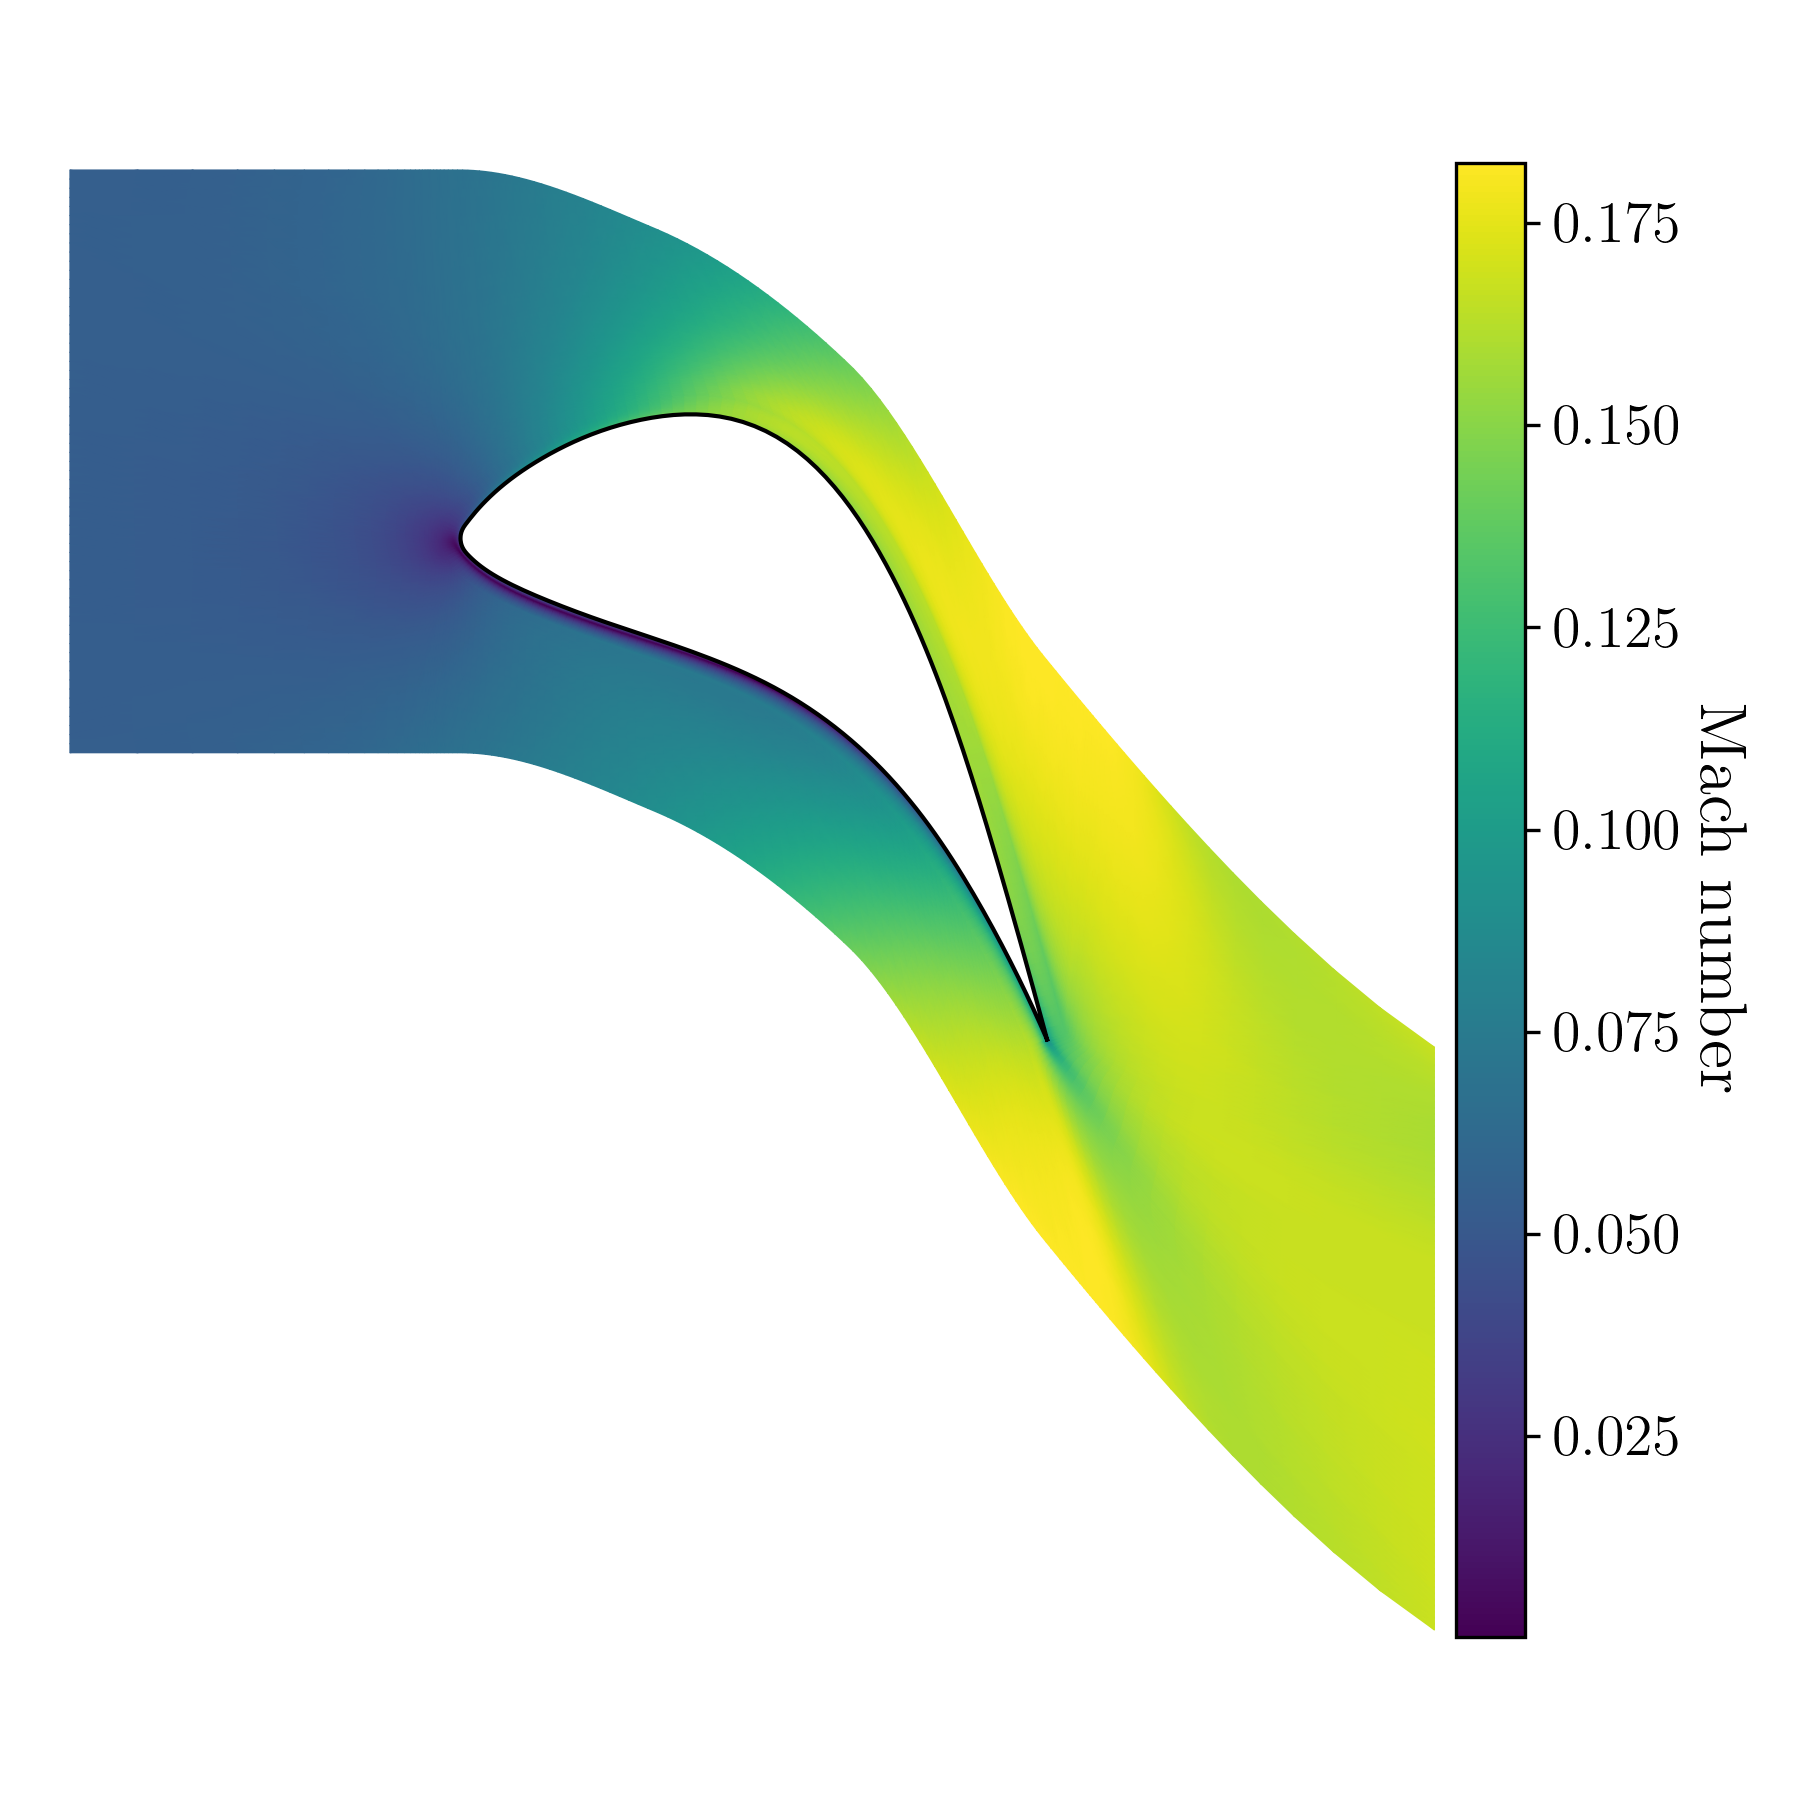
\includegraphics[width=0.99\textwidth]{figures/turbine_c_mach.png}
        \caption{}
        \label{fig:turbine_c_mach}
    \end{subfigure}
    \caption{Turbine\_c test case results}
\end{figure}

\begin{figure}[H]
    \centering
    \begin{subfigure}{0.46\textwidth}
        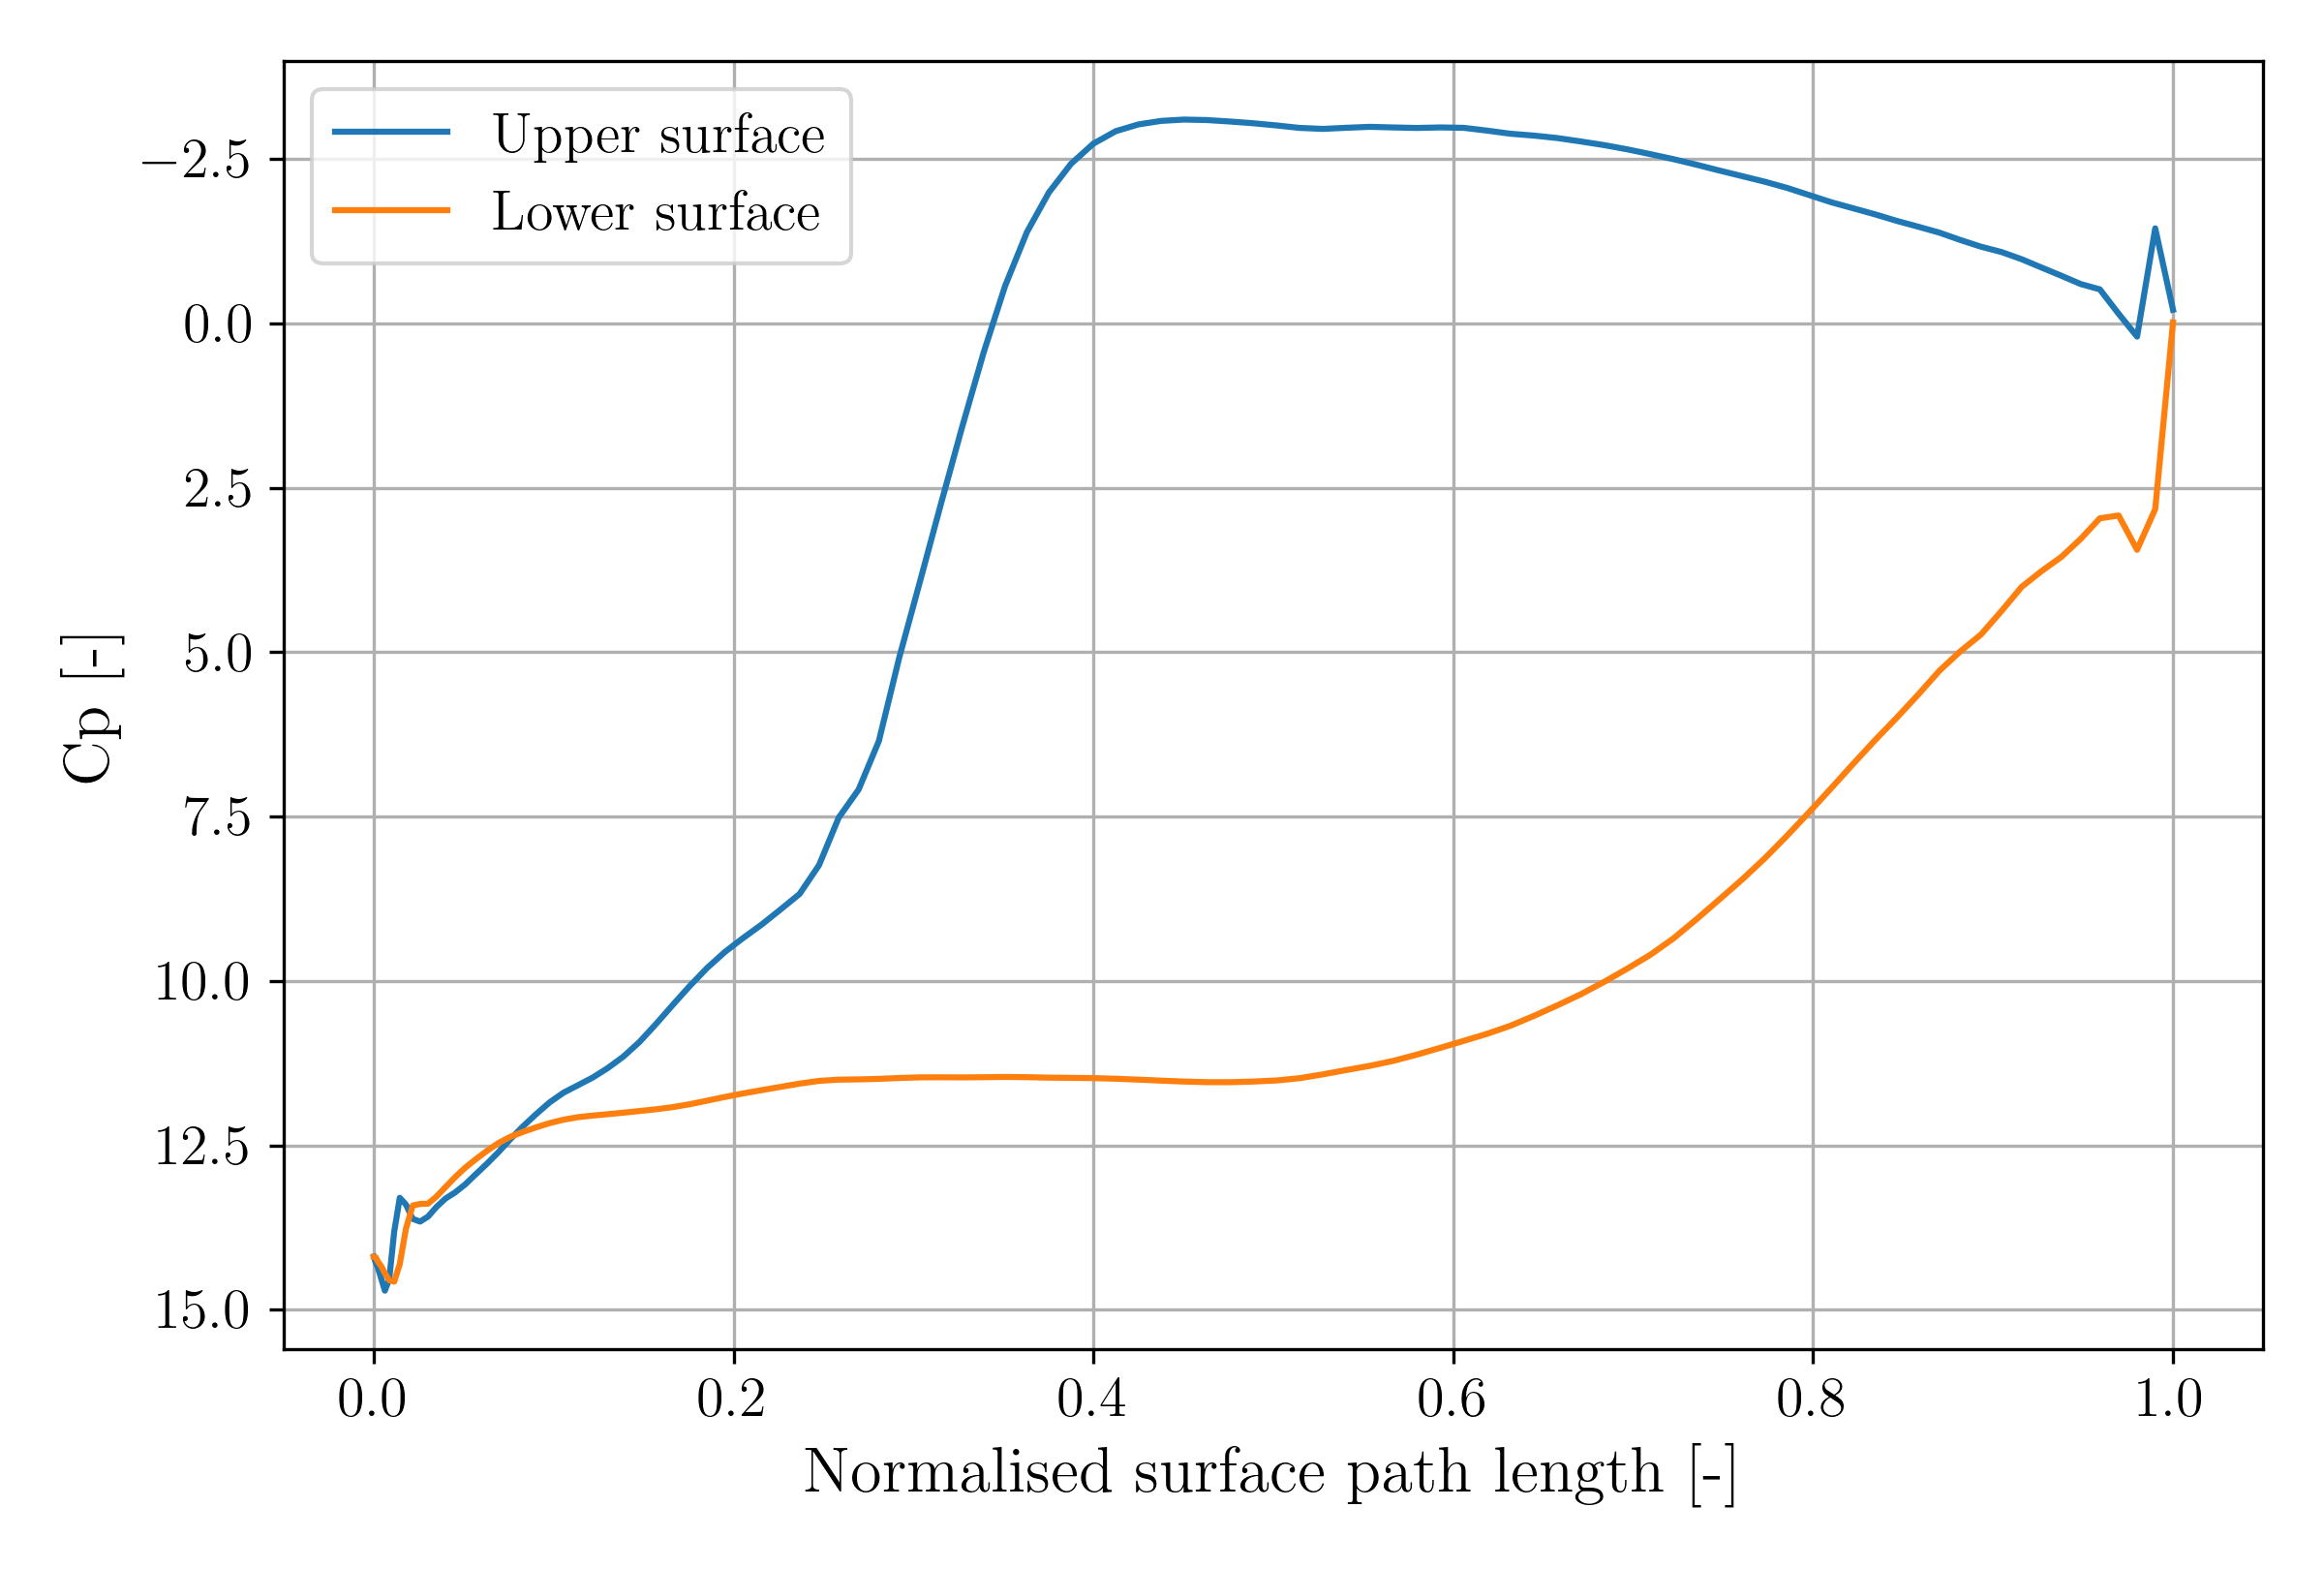
\includegraphics[width=0.99\textwidth]{figures/turbine_c_surface_cp.png}
        \caption{Turbine\_c test case results}
        \label{fig:turbine_c_surface_cp}
    \end{subfigure}
    \begin{subfigure}{0.5\textwidth}
        \centering
        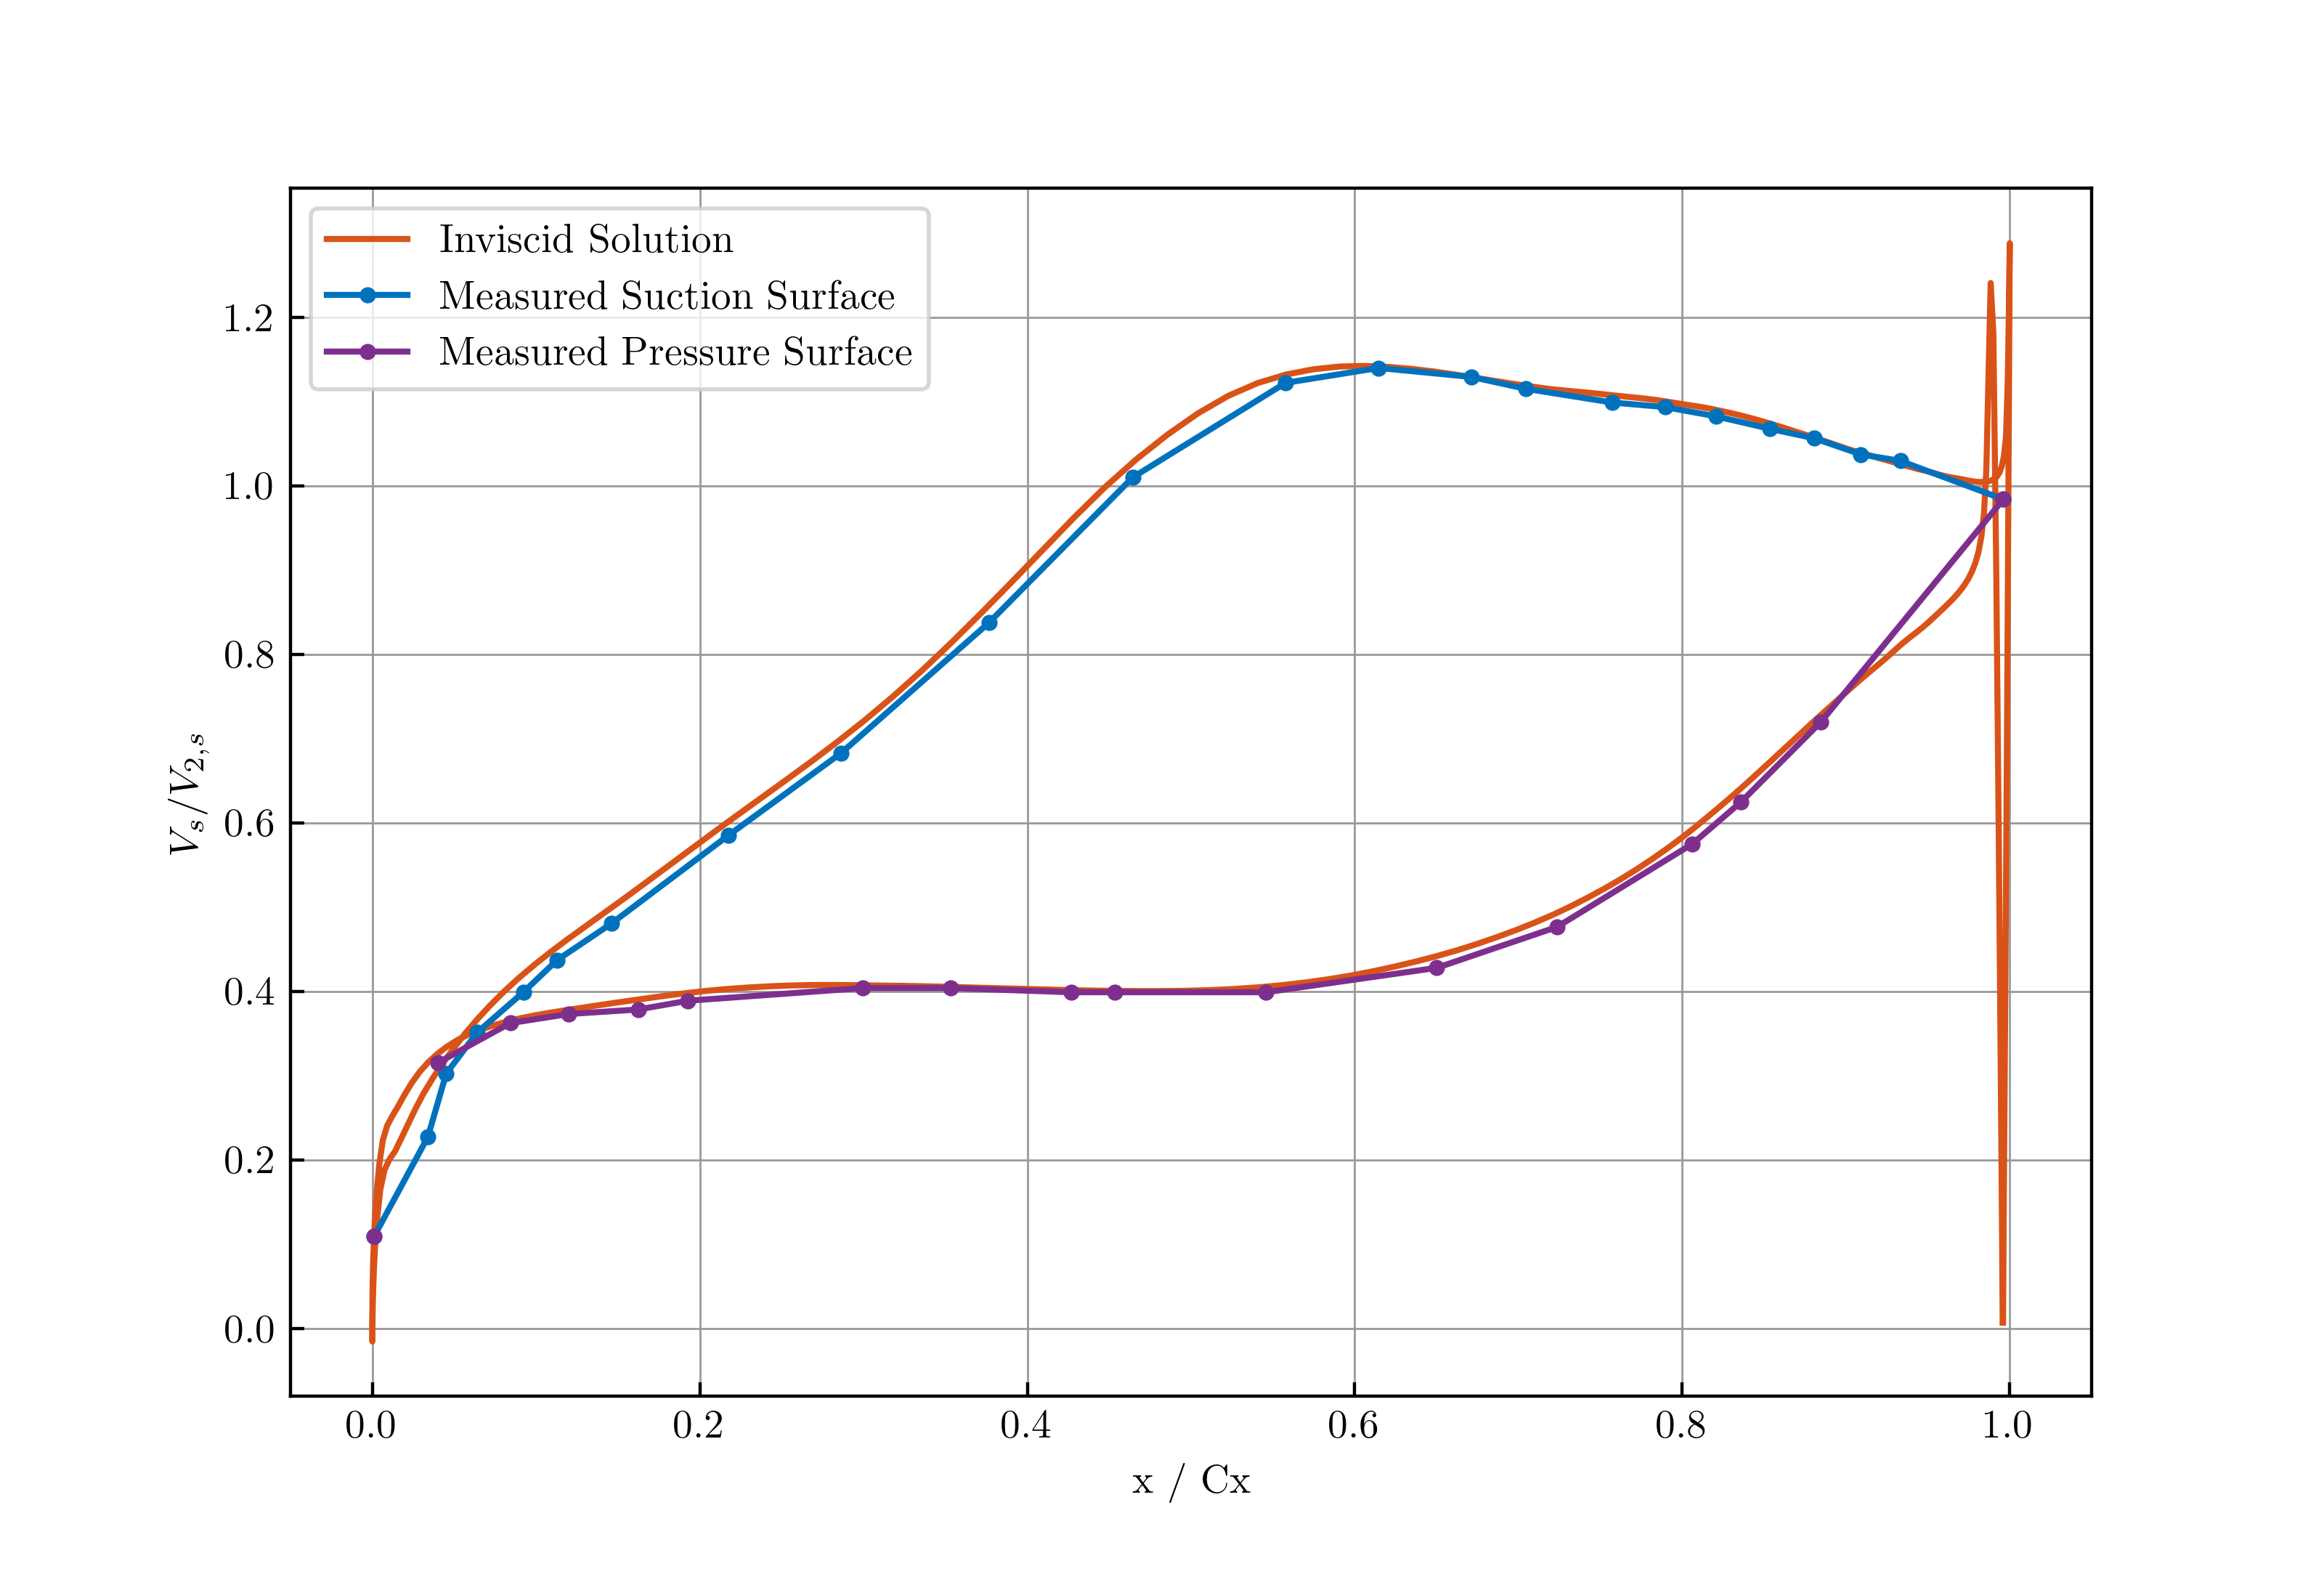
\includegraphics[width=0.99\textwidth]{figures/turbine_real.png}
        \caption{Real turbine data \cite{4A3_lab}}
        \label{fig:turbine_real}
    \end{subfigure}
    \caption{Comparison of CFD to experimental data}
\end{figure}

\subsection{Effort vs Accuracy}

\section{Discussion}
% two pages that doesnt repeat interim

\subsection{Naca airfoils}

Figure \ref{fig:cl_alpha} shows the lift coefficient against angle of attack for the Naca0012 and Naca2412 airfoils.
From invicid theory, these lift coefficient should be linear with angle of attack with gradient $ 2\pi $. ( our algorithm can now compute PI !)
The actual gradient observed is 4.5\% higher than $2/\pi$ for the Naca0012 and 10.9\% lower for the Naca2412.
Why?

\subsection{Turbine}

The turbine case had very similar mesh geometry to 

\section{Summary}

\section{References}

\begin{thebibliography}{9}

    \bibitem{handout}
    J. V. Taylor
    \emph{4A2 Computational Fluid Dynamics: Writing an Euler Solver}
    University of Cambridge,
    2024.

    \bibitem{solve_ODE_nonstiff}
    Hairer, Ernst et al.
    \emph{Solving ordinary differential equations I: Nonstiff problems, Berlin, New York}
    Springer-Verlag, Berlin(1993)

    \bibitem{4A3_lab}
    L. W. Pender
    \emph{4A3 Turbomachinary Laboratory Report}
    University of Cambridge,
    2024.
  
\end{thebibliography}

\section{Appendix}

\subsection{Worker runtime enviroment}

A worker directory folder is created in the following format:
% directory tree for bump worker
\begin{figure}[H]
    \dirtree{%
    .1 1.
    .2 bump.
    .3 input\_bump.txt.
    .3 conv\_bump.csv.
    .3 out\_coord\_bump.bin.
    .3 out\_final\_bump.bin.
    .3 geom\_bump.txt.
    .3 out\_guess\_bump.bin.
    .2 log.txt.
    }
    \caption{Worker directory structure}
    \label{fig:worker_dir}
\end{figure}

During setup \texttt{generate\_case} is called and the settings and geometry files are written to the case folder.
During runtime the \texttt{log.txt} acts as \texttt{stdout} for the program.
When the solver finishes then the out files are saved and processed using the postprocessing python functions.

\begin{lstlisting}[language=Python]
def run(self):
    self.setup_environment()
    with open(self.log_file, "w") as log:
        try:
            parsed_file = str(self.in_file).replace("\\", "/")
            t1 = time.time()
            subprocess.run([self.cfd_executable, "--path", parsed_file],
                            check=True,
                            stdout=log)
            t2 = time.time()
        except subprocess.CalledProcessError as e:
            print(f"Worker {self.worker_id} failed with error: {e}")
            return

    self.dt = t2 - t1
    results = self.parse_results()

    # Write results to the shared file in a thread-safe way
    with self.shared_lock:
        with open(self.shared_file, "a", newline="") as csvfile:
            writer = csv.writer(csvfile)
            writer.writerow(results)

    print(f"Worker {self.worker_id} finished.")
\end{lstlisting}

\subsection{Identical turbine geometry}

\begin{figure}[H]
    \centering
    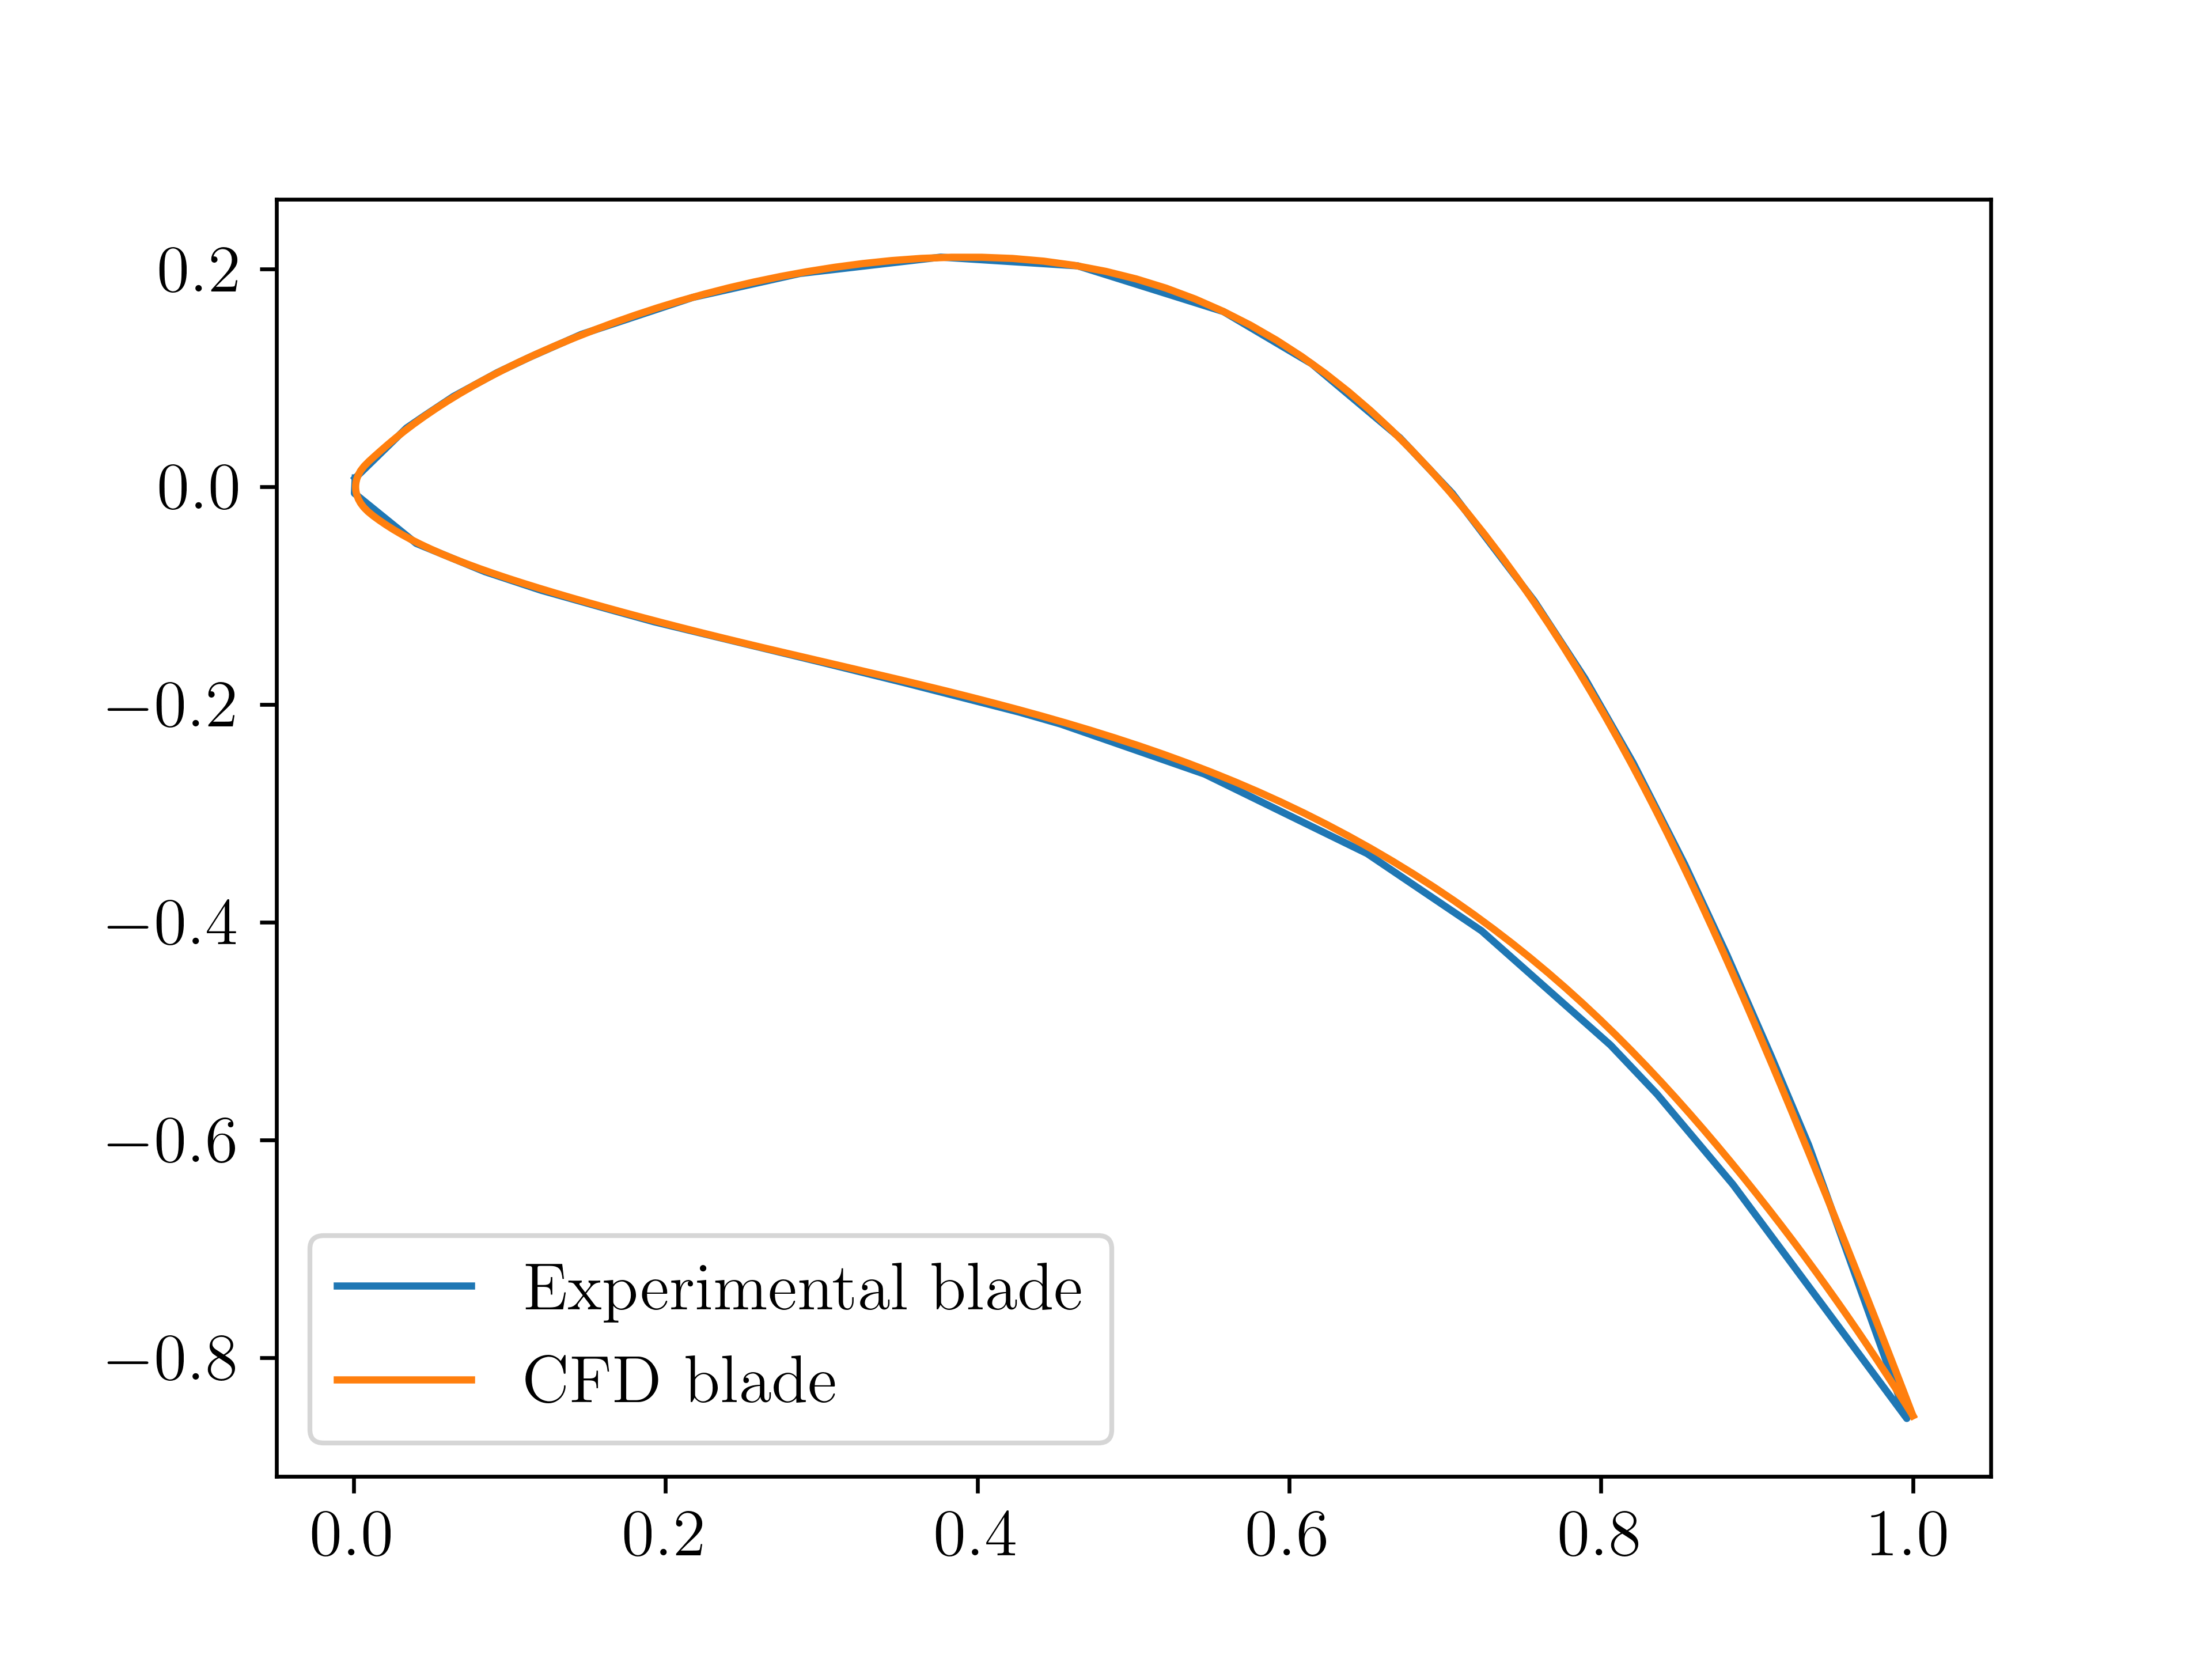
\includegraphics[width=0.6\textwidth]{figures/turbine_geometry.png}
    \caption{Comparison of turbine geometry}
    \label{fig:turbine_geometry}
\end{figure}

\end{document}